\documentclass[12pt,letterpaper,table,svgnames,dvipsnames]{article}

% \begin{preamble}
\usepackage[margin=1in]{geometry}
% \usepackage{times}
\usepackage{helvet}
\renewcommand{\familydefault}{\sfdefault}

\usepackage{apacite}
% \usepackage{dblfloatfix}
\usepackage{caption}
\usepackage{subcaption}
\usepackage{graphicx}
\usepackage{tcolorbox}
% \usepackage{multicol}
\usepackage{makecell}
\usepackage{xcolor}
\usepackage{booktabs}
\usepackage{url}

% To keep track of total pages
\usepackage{fancyhdr}
\usepackage[page]{totalcount}
\pagestyle{fancy}
\fancyhf{}
\cfoot{Page \thepage~of \totalpages}

\usepackage{gb4e}
\noautomath
% \end{preamble}

\definecolor{Purple}{RGB}{255,10,140}
\newcommand{\jd}[1]{\textcolor{Purple}{[jd: #1]}}
\newcommand{\mm}[1]{\textcolor{teal}{[mm: #1]}}
\newcommand{\tableref}[1]{Table~\ref{#1}}
\newcommand{\figref}[1]{Fig.~\ref{#1}}
\newcommand{\expref}[1]{Exp.~#1}
\newcommand{\whq}{\emph{wh}-question~}
\newcommand{\whqs}{\emph{wh}-questions~}
\newcommand{\whw}{\emph{wh}-word~}
\newcommand{\whws}{\emph{wh}-words~}


\title{\textbf{On the (non-)exhaustivity of naturally occurring \whqs}}
\author{\Large{Morgan Moyer \& Judith Degen}\\
Universit\'{e} Paris-Cit\'{e}, Stanford University}
\date{\today}

\begin{document}
\maketitle

\begin{center}
    \textbf{Abstract}\\
    Blah blah blah
\end{center}

\section{Introduction}

A root \whq can be answered in multiple ways. 
% \vspace{-.3cm}
\begin{exe}
    \ex {}
    \begin{xlist}
        \ex Where can I find coffee? \label{coffee1}
        % \vspace{-.1cm}
        \ex Who came to the party? \label{party}
    \end{xlist}
\end{exe}
% \vspace{-.3cm}
The most natural way to answer (\ref{coffee1}) is to mention a nearby coffee shop, while the most natural way to answer (\ref{party}) is to provide an exhaustive list of party-goers. That is, out of the blue, (\ref{coffee1}) receives a \emph{non-exhaustive} interpretation, while (\ref{party}) receives an \emph{exhaustive} one. We refer to these readings as `Mention-Some' (MS) and `Mention-All' (MA), respectively \cite<following> {hintikka1976,groenstok1982,groenstok1984}. MS and MA are also available as possible readings of embedded \whqs$\!$:
\begin{exe}
    \ex {}
    \begin{xlist}
        \ex Scully knows where I can find coffee. \label{emb_coffee1}
        % \vspace{-.1cm}
        \ex Scully knows who came to the party. \label{emb_party}
    \end{xlist}
\end{exe}
(\ref{emb_coffee1}) is true if Scully knows an MS answer to the root question (\ref{coffee1}), while (\ref{emb_party}) is true if Scully knows an MA answer to the root question (\ref{party}). On the surface, \whqs do not specify whether they are intended to be MS or MA. What makes (\ref{coffee1}) and (\ref{emb_coffee1}) naturally MS, and (\ref{party}) MA? 
% The answer to that question is the focus of this paper. \jd{we don't provide a full answer, so might have to weaken} 
In this research, we offer a contribution to answering that question by looking at the distribution of MS and MA interpreatations in naturally-occurring \whqs$\!$.

We will use the term `interpretation' to refer to the final MS or MA reading that a hearer lands upon in a context. The MS interpretation in (\ref{coffee1}) is licensed by contextual goals \cite{groenstok1982,groenstok1984}: if (\ref{coffee1}) is asked by a tourist whose goal is to drink a coffee, then an MS interpretation is more felicitous; if asked by a coffee distributor whose goal is to explore the local market, then an MA interpretation is more felicitous.
% \jd{presumably, MA is felicitous one way or another? perhaps "more felicitous" instead of just "felicitous" in both cases?}. 
% \mm{That's what we assumed in the study from my dissertation looking at high/low stakes. It was another implicit assumption in the literature. I think van rooij is the only one where that was almost explicitly discussed. However, we found in low stakes that MA was actually \emph{less} felicitous. That was a surprising result. Though Yimei's response was that actually MA answers were really mixed T an F cases there (cause implicit ordering should pick out only the best answer, and MA answer contains non-best answers).}
However, not all \whqs lend themselves to MS, while MA appears to be available for most (if not all) \whqs. Indeed, (\ref{party}) is often presented as a paradigm \whq that does not allow MS.
% \jd{again, sloppy use of "MS/MA" -- either define it to mean "Mention-Some interpretation/answer", or write expclitly "...that does not allow an MS interpretation/answer"}.

Previous work on the availability of MS/MA interpretations of \whqs has typically focused on a small number of examples passed down through the literature, on the implicit assumption that \whqs do not vary greatly. \cite{}
% \jd{mention refs here (include many so individuals don't feel unduly attacked)} 
Recent work the availability of MS/MA experimentally has systematically varied both linguistic and contextual factors across a broader range of sentences and contexts, with the goal of creating a more stable empirical basis for a theory of \whq meaning \cite{moyersyrett2019,moyer2020}. That work has revealed that the availability of MS/MA is a function of both linguistic form of the questions and the speaker's contextual goal. 
% \jd{perhaps provide example, and how this contrasts with the previous literature? because above you already say speaker goals matter, so what's different here? at this point it needs to be clear what the issue is that there is still uncertainty about.}
On the one hand, while questions without modals are on average less acceptable on MS readings, explicit non-exhaustive discourse goals (for example, searching for a cup of coffee as compared to searching for people trapped in a burning building) can actually bolster the acceptability of a MS interpretation of such non-modal questions. On the other hand, MA interpretations can be equally \emph{infelicitous} when discourse goals are non-exhaustive. The flexibility of interpretation in both directions has often been overlooked in the literature, with the exception of \citeA{ginzburg1995,asherlascarides1998,beckrull1999,lahiri2002}. In part, this could be due to the focus on a select few of examples, and the methodological attempt to separate out the effect of context. We discuss this methodological point in section XXX. 


% \jd{i tried to fix this up a bit, but before we even say what we did, readers need to expect us to do that -- so the role ling form vs context dichotomy needs to be set up better above; we can discuss}

% The picture that emerges is that there is considerable variation in \whq interpretation. That variation is the result of (1) inferred contextual goals of the speaker \jd{do we test this explicitly? how? here we should really only list what there is hard evidence for, and not speculation}, (2) the uttered question \jd{do you mean linguistic surface features? if so, say so}, (3) the hearer's inferences about the two \jd{how are the inferences different from the factors? probably delete this point, unless you quantify the inference separately in some way?}, and (4) any prior expectations that the hearer might have about either (1), (2), or (3) \jd{again, is this speculation based on individual examples cherry-picked at the end? or is this a clear empirical result? it's fine to just discuss these issues at the end, or foreshadow that you'll discuss them, but avoid presenting things as fact that aren't}. Together, with a more qualitative analysis of the contribution of the preceeding discourse context we argue that accounting for \whq meaning in terms of MA , or in terms of exceptional linguistic forms \jd{what is "accounting for \whq meaning in terms of MA, or in terms of exceptional linguistic forms" supposed to mean? vague.}, ignores important generalizations about non-linguistic information.


% \jd{given all the listed issues with the previous paragraph, i suggest replacing it with something like the following: "The picture that emerges is that there is considerable variation in \whq interpretation. That variation is the result of both linguistic form factors (e.g., ) and additional contextual factors (e.g., XXX). We argue that MS licensing is not an exceptional fringe phenomenon, and that, instead, a theory of \whq meaning will have to account for the interplay of semantic and pragmatic factors."}



% \jd{if we're still making the "here is the maximal semantic claim we can make on the basis of the data" point, this is where it should be foreshadowed.}


In the next section, we will discuss both the main theoretical treatments of Mention-Some, and review the factors which have been observed to affect the distribution of this reading, the presence/absence of modals, the wh-word, and matrix embedding verbs for embedded questions. We will then summarize with the main predictions derived theoretically and from observation of the literature. 

In the current study, we test which claims about MS/MA licensing previously made on the basis of a few hand-selected or artificially constructed examples generalize to thousands of naturally occurring \whqs$\!$. We operationalize the availability of MS and MA interpretations via the acceptability of question paraphrases elicited in a paraphrase rating task. Experiments 1 tested root (Experiment 1a) and embedded (Experiment 1b) \whqs in their immediately preceding discourse context (Section XX). We find that some but not all predictions from the literature are borne out, and in particular we find no overwhelming MA bias, but we do find modulation of interpretation based on both Wh-word and modality, and matrix verb to some extent. In section XXX we present a second set of studies (Experiments 2a and 2b), using the same stimuli and task as the first two experiments. Crucially, in these studies we presented participants with target questions \emph{without} their discourse contexts. Surprisingly, and in stark contrast to the literature predictions, we find significant bias for MS interpretations, although overall participants were more uncertain about the distributions of question meanings. As for our other factors of interest, we still find effects of wh-word and modality, although to a much lesser degree.

The picture that emerges is that there is considerable variation in \whq interpretation. That variation is the result of both semantic (e.g., the presence/absence of existential modality, or the question-embedding verb in the case of embedded questions), and additional pragmatic factors (e.g., the resolution of the \emph{wh}-domain, and the role of contextual discourse goals). We argue that MS is not an exceptional fringe phenomenon, and that instead, an adequate theory of \whq meaning will have to account for the interplay of both kinds of factors. On this basis of our data, we think that the maximal semantic claim that can be made is that questions are generally either ambiguous or underspecified for MS or MA, but that other factors like the presence of existential (modal) force, the pragmatics associated with resolving the \emph{wh}-domain and reasoning under uncertainty about the speaker's goals, drive hearer perceptions about (non-)exhaustivity in \whqs $\!$. 



\section{Mention-Some and the semantics/pragmatics of \whqs}
% \jd{this and the "treatment of MS" section should probably be merged. and probably moved before the linguistic and contextual factors sections. otherwise the factors sections contain terms that haven't yet been introduced. also, make sure to only include information that is relevant to the main argument. you don't need to provide an exhaustive list of everything anyone has ever said about questions; you just need to give the reader the information they need to understand the argument}

% \jd{in general, this whole section reads as a chronological "this person said this and then this other person said that" -- completely restructure to give the reader a sense of a) what is the most basic semantics of root questions that we endorse; b) what is the most basic semantics of embedded questions that we endorse? c) what are the consequences of these proposals for the availability of MS/MA? d) what are the dimensions along which current theories of wh-questions differ, such that they make possibly different predictions for MA/Ms availability? eg, it sounds like some accounts of MS/MA are ambiguity accounts, others are underspecification accounts. if so, say so. here you also talk about different levels of exhaustivity, which are not mentioned in the intro. do you want to introduce these levels directly? if so, related them to how you're thinking about MS/MA availability as laid out in the intro.}

The theoretical landscape with regards to the semantics/pragmatics of \whqs is highly disputed, and it raises theoretical and empirical issues that extend farther beyond the topic of \whqs. There are consistent empirical observations which can and are explained in theoretically conflicting ways; even the data themselves are questioned. That makes a straghtforward disucssion--and theory testing--approach difficult, to say the least. 

% When you can't take the data at face-value,
% A common starting place for a discussion is with \citeA{hamblin1973}, who proposed that a question denotes the set of its possible answers. This theory and particularly its later kin

% The MS reading is even weaker than the weak exhaustive reading. Intuitively, the MS reading is existential, and the MA is universal \cite{hintikka1976}\mm{double check date}. 

With that being said, we can say that there are two simple ways to approach MS: either it is semantic or it is pragmatic. Semantic treatments aruge that there is an underlying semantic explanation for MS, in other words that MS is grammatically licensed. In contrast, pragmatic accounts argue that pragmatic factors explain MS. This is a classic juxtaposition.

What are pragmatic factors? For Karttunen and Groenendijk \& Stokhof, it means a non-truth conditional process that determines what counts as a good answer (see, \citeA{karttunen1977} footnote 4; \citeA{groenstok1984} footnote 14 and discussion pp. 533). This understanding of ``pragmatic'' is maintained in \citeA{george2011} and indirectly in \cite{xiang2016} in the form of arguments against embedded ``pragmatic'' MS. The idea is that what counts as a good answer depends on the speaker/hearer interests, and in the embedded case, this information cannot penetrate grammatical structure. For Asher \& Lascarides and Ginzburg, ``pragmatic'' implies information about a conversational participant's beliefs/cognitive state, and goals/plans \cite<seee discussion on pp. 266 of>{asherlascarides1998}. The difference between these two perspectives is whether this pragmatic information has truth-conditional repurcussions; whether this information is available to the internal knowledge representations involved. 

The problem here, is that drawing the line based on truth-conditional effects doesn't actaully aid either the empirical or theoretical situation. This is because of context-sensitivity.


% Let's look at analogy from a different field. It was long assumed that humans made (economic) decisions following the mathematical tenents of probability theory. The field of Behavioral Economics arose exactly because there was a discrepancy in the data: probablilty theory predicted 


Drawing a distinction in this way confounds two separate perspectives on language \emph{understanding} and linguistic theory. Both present useful insights into how a \emph{hearer} determines the meaning of a \whq, but crucially make different assumptions about both theory and data. By introducing these perspectives, we will provide a frame in which to elaborate on our own view on MS and \whqs.

In his 1992 book \emph{Arenas of Language Use}, Clark described two approaches to linguistic inquiry: the language as \emph{product} approach and the language as \emph{action} approach. Product traditions view the sentence as a basic unit, an abstract representation produced by a grammar. In the realm of semantics, a semantic theory follow the product tradition, abstracting away as much as possible from any circumstantial or indexical information. Groenendijk \& Stokhoff allude to this in footnote 14 of the 1984 joint-dissertation, which describes their motivation for the semantics/pragmatics divide that they assume. Additionally, this thinking seems to underly George's rejection of a van Rooij style semantic theory, which supposedly gives up simplicity for incorporating more contextual/intentional/mental state information into the semantic theory (discussion on p.205). Often, such contextual information is acknowledged as playing a role in language production and comprehension, but then disregarded as playing a role in determining the truth (or answerhood) conditions of \whqs. It has often gone hand-in-hand with the idea that pragmatic information cannot ``interfere'' with semantics, and thus the prediction that MS should not occur in (at least some) embedded questions--see also \citeA<footnote 4>{karttunen1977}, and \cite{xiang2016}\mm{page number}.


In contrast to product theories, action traditions follow in the steps of speech act theorists and ordinary language philosophers like Austin, Searle and Grice. These traditions hold utterances to be the more basic unit, and therefore equally important to the sentences which they token, are the contextual circumstances in which they are tokened. This includes indexical information about the speaker, hearer, goals. Utterance `meaning' then refers to what Grice and Austin called `speaker meaning', and is guided by the recognition of speaker and hearer intentions. It's possible that theories along the lines of Ginzburg and Asher \& Lascarides would be candidates for being considered action theories, because their analyses of \whqs are parts of the analyses of dialogue more generally, often appeal to situational information like cognitive states and plans. 

In this work, we adopt the perspective of the langauge as action tradition. Our guiding inquiry, then, concerns the \emph{interpretation} of \whqs, which happens by necessity in fixed naturalistic contexts, with conversational agents present, and actively engaged (presumably) in cognitive processes like mind-reading/intention-recognition. We will treat semantic theories as presenting minimal models of the conditions on interpretation. The linking assumption is that, if a theory puts a mechanism in the semantics, the reason is because that mechanism is by hypothesis part of the basic meaning of the linguistic item in question. Thus, by convention, this predicted semantic component presumably should be borne out more often than not empirically---that is, in the interpretations that na\"ive language users access on average. The behavioral patterns that we see in na\"ive language users should reflect the presence of the hypothesized mechanism.

With these comments in mind, we turn to the behavioral patterns that the semantic theories above predict when it comes to \whq interpretation. 

In the following sections, we discuss the approaches to MS, and in the process identify four critical observations about factors that modulate the interpretation of MS, and \whqs generally. These four factors have served differentially as evidence for semantic and pragmatic accounts of MS, thus our discussions of theory will be tied up with the evidence that has been produced in support of those theories. To preview, the effect of existential (modal) force, and matrix question-embedding verbs will unroll in the section on semantic theories of MS; while the effects of \whw and contextual discourse goals will be discussed in the section on pragmatic approaches. 

% Since then, many semantic theories have worked with some version of this hypothesis, and variations arose (and continue to arise) from disputes about exactly \emph{which} answers should count as ``possible answers'' \cite<e.g.,>{karttunen1977,groenstok1982,groenstok1984,heim1994,beckrull1999,george2011}. 


% The predominant focus in this research has been on degrees of MA, that is weak, intermediate, and strong exhaustivity \cite{karttunen1977,groenstok1982,groenstok1984,heim1994,beckrull1999,sharvit2002,guerzoni2007,guerzshar2007,george2011,nicolae2014,uegaki2014,uegaki2015,theiler2014,roeltheilalon2014}.\mm{get all the cites} Briefly, a weak exhaustive answer/reading picks out only the true answers to the question, while strong exhaustivity imposes a further condition that those are the only true answers. Finally, intermediate exhaustivity is weak exhaustivity plus a condition that the answerer or agent of the embedded question report has no (false) beliefs that any false answers are true \cite{spector2005,klineroth2011}. For our purposes, we will refer to these all simply as MA, and not distinguish them unless a distinction becomes necessary.

% It is worth mentioning that, while the approaches above represent common theoretical starting points for a semantics of questions, there are other approaches which have focused on different aspects questions. For example so-called functional theories (cf. \cite{krifka2011}) ...


% This kind of partitioning raises an orobourus. It isn't straight-forward what it means to be semantically licensed or not. Some theories provide semantic explanations via context-sensitive operators/variables which determine the truth conditions of \whqs (cf. \cite{lahiri2002,vanrooij2003,vanrooij2004}). In the sense that the operator/variable is present in the semantic representation they should be considered semantic theories; however, they are typically classified as pragmatic because context must provide the value of the variable/operator. In contrast, more standard theories like \cite{beckrull1999,george2011,fox2014,nicolae2014,xiang2016},\mm{fox 2018,xiang 2020?} which posit lexical or syntactic ambiguity are considered semantic, even though ambiguity relies on contextual disambiguation (see discussion in \citeA{groenstok1984} p. 544, \citeA{dayal1996} pp. 61). In both these cases, the predicted behavior would be the same.

% Relatedly then, once you admit context-sensitivity, inferring an underlying theory from any acceptability judgement is nearly impossible. If a semantic theory accounts for MS via appeal to an ambiguity, then that ambiguity will be resolved in context, and give the appearance of context-sensitivity the same as the pragmatic accounts which argue that MS arises via some appeal to contextual goals (regardless of the underlying semantic representation). 


% This is also not to say that \emph{all} semantic theories see themselves as product theories. This is not to say that there are no product-type semantic theories which attempt to deal with context-sensitivity. In fact, there is a wealth of research on this very topic, and it often straddles the disciplinry boundaries of philosophy of language and semantic theory. Sometimes the terms ``metasemantics'' is applied to theories that deal with licensing of variables. \mm{For example, Kaplan's 2-D semantics for demonstratives, Stanley and Szabo...King...} There are also more linguistic cases, like work on gradable adjectives (\mm{refs}), vagueness (\mm{}), 

% Of course, interpretation will ultimately be a mix of semantics and pragmatics given its situated-ness (\mm{does the evoke the wrong backgound of literature?}).

% There are some exceptions to the claim that linguistic theories typically fall in to the language as product view as articulated above with respect to contextual information---i.e., not all product theories ignore contextual information. Semantic theories that deal with context-sensitive phenomenon, like vagueness, ambiguity, genericity, polysemy, reveal the challenges of separating meaning from context of use. Context-sensitivity can be accounted for in the grammar by a language-as-product theory often by appeal to formal devices like varibles (pronouns) whose referents are fixed only in a context. For example, Kaplan's influential 1989 theory of indexicals made headway in the formal treatment of indexical expression, and has been the basis for other theories of context sensitivty. 

% The grammar may constrain a variable's referential domain, but human psychology takes care of reference resolution in a given context. How a given hearer resolves a given varible isn't necessarily the concern of the product theorist. 

% Chomsky (\mm{1965}) aruged that linguistic theory should describe the competence or, abstract knowledge system, of an ideal speaker/hearer, and not the way language is used in communication. This competence/performance distinction still guides contemporary linguistic inquiry, but in the domain of the semantic-pragmatics interface the distinction is less clear. Some may argue that to take a semantic theory about abstract question meaning and derive predictions about how hearers will interpret a question in a dialogue context is a theoretical category mistake which may mislead the researcher to draw incorrect conclusions about question meaning.


% \mm{useful exercise for us to flag whether each theory comes from the action versus product. The ones under product are there because they crucially appeal to context in ways that the others do not. Although there's some ambiguity because Lahiri's account is very product oriented, but he appeals to contextual variables as well to fix semantic content. I'd say that most fall into the product box, with the exception of the ones in action.}
% \begin{figure}[h!]
%     \centering
% \begin{tabular}{|l|l|}
%     \hline
%     Action theory & Asher \& Lascarides, Ginzburg, van rooij, Lahiri? \\
%     \hline
%     Product theories & Karttunen, G\&S, Lahiri, Fox, Nicolai, Xiang, Beck \& Rullmann, George\\
%     \hline
% \end{tabular}
% \end{figure}

% \begin{itemize}
%     \item \citeA{george2011}, pp. 201: ``The second issue [with an ambiguity account] is that it seems likely that [it] overgenerates: there are few cases where a single embedded question clearly has access to both readings, and a number of cases where only one reading appears to be present,'' 
%     \item Fox 2014, p.3: `` Disadvantages of [George 2011's] Theory 1: doesn't capture the limited distribution of MS readings (pointed out by George)'' 
%     \item Fox 2018 in section 4 (pdf p.12): ``With a more sophisticated theory of exhaustification (one that accounts for the conjunctive interpretation of disjunction in certain modal contexts), we will see that the MS/MA ambiguity can be attributed to an ambiguity in the question denotation.''
%     \item fox 2018: discussion section 5 pdf pp21: suggests thaat non-existential cases of MS are really implicit domain restriction (Spector 2018 arguing this for weak exhaustivity?)...page 24, about example (45b): MS is harder to get. also Section 7 p. 27, ``not sufficient to constrain MS''
%     \item include Chierchia and Caponigro (2013) (reference from Fox 2018)
%     \item Dayal (2016), 75: ``The primary thrust of our investigation so far has been on exhaustive answers, which are generally taken to represent the unmarked case.''
%     \item Xiang, under review paper, pp.16: ``Assumptions made in this section cannot fully explain why MS interpretations are \emph{only} available in \emph{can}-questions.'' (maybe better to look at published paper form 2020)
%     \item debate about what is MS, modals or anything existential?
%     \item van Rooij (2004), p. 10: ``this suggests that a \whq will usually get a mention-all interpretation, because usually the question has a utility that is strictly higher on this interpretation.''
%     \item Nicolae (2013), p.177: we have been assuming questions are exhaustive, but that's not the case when there's an existential...
%     \item Xiang \& Cremers (2017): opening para: ``In most daily conversations, a question admits only an exhaustive answer.''
% \end{itemize}
% Nicolae (2013), p.17, 
% Fox 2014, p.3
% Fox 2018 in section 4 (pdf p.12)
% Xiang, under review paper, pp.16
% Xiang \& Cremers (2017)
% \citeA{george2011}, pp. 201
% van Rooij (2004), p. 10

% Dayal (2016), 75

% \noindent No embedded pragmatic mention-some
% \begin{itemize}
%     \item ``Framed in Gricean terms, [a pragmatic] response has a serious flaw: it cannot account for the availability of mention-some readings in embedded questions,'' (\cite{george2011}, pp. 204)
%     \item van rooij (2004), pp.5
%     \item G\&S: footnote 14
% \end{itemize}


\subsection{Semantic treatments of MS and predictions about the distribution of MS and MA}


Many researchers have implicity assumed that MS is more limited in distribution than MA, assuming that the predominant reading/answer is MA in most cases. As a result, many have maintained theories which posit only an underlying MA semantic representation usually based off \citeA{karttunen1977} or \citeA{groenstok1982,groenstok1984}. Some places where this view is explicitly stated \cite[Ch.6]{groenstok1982,groenstok1984,karttunen1977,vanrooij2003,nicolae2014,fox2014,xiang2016,dayal2016,george2011}.\mm{xiang2020,fox2018}. 

% The importance of existential elements has been demonstrated by experimental work showing that MS is more acceptable with modal than with non-modal questions  \cite{xiangcremers, moyersyrett2019}. This gives rise to the first empirical observation that we aim to test: that existential modal questions give rise to a greater rate of MS than non-modal questions.


% \jd{the received wisdom observations that MS distribution is limited should be merged into the end of the theory section (together with the "disagreement about the representation of mention-some" section below. there's a lot in that section that is redundant with what is already in the theory section, and other things -- like the nice setup of different dimensions along which accounts differ with respect to how they handle MS vs MA -- that is really needed in the theory section) and moved before the factors section. any observations about individual factors affecting MS should be merged with the various factors sections}

Thus, if the bare semantic contribution of a \whq is MA, then on average, we should find MA interpretations rated higher than MS interpretations. Additionally, we should find that MA interpretations will persist (or even increase) reqardless of whether contextual information is provided.
% \mm{review bernhard schwarz 2017 paper}

\begin{tcolorbox}[colback=white]
\noindent \textbf{Prediction 1: General MA bias}. \\
MS is limited in distribution, but MA is availble for all \whqs.
\end{tcolorbox}

% What about mention-n readings (Xiang 2016 and Fox 2018 discussion of that pp 27)?
% \mm{this is disucssion where it will be relevant to distinguish degrees of MA just to do somewhat justice to this literature, since here has been so much focus on MA rather than MS.}

Despite this often implicit assumption, there are those who argue for ambiguity in \whqs. Theories like \citeA[Ch. 2]{hintikka1974,berman1991,berman1994,beckrull1999,lahiri2002,george2011} \mm{make sure the IS citations are correct} \cite{ciardelliroelthei,ciargroroel,theiler2014,theiroealo2016} posit that all questions in principle can allow for MS or MA.\footnote{Theories like \cite{ginzburg1995,asherlascarides1998,vanrooij2003,vanrooij2004} also make this claim that in principle all questions should all MS and MA. We categorize these theories however as pragmatic because the explanatory brunt behind what makes a question MS or MA is going to crucially involve pragmatic information. At the same time, the same will be true of so-called semantic theories that posit ambiguity, because contextual factors are implicated in disambiguation.} For instance, Hintikka originally argued that questions were ambiguous between existential (MS) and universal (MA) readings. \citeA{beckrull1999} aruge that there is a range of readings available for \whqs and thus that the semantics should provide the tools to account for that. Their theory posits several different type-shifting answerhood operators (following \cite{heim1994}). They acknowledge that the final interpretation will be determined by the pragmatics of disambiguation. \citeA{lahiri2002} agrees, though his operator includes (i) a context sensitive variable to allow for restrictions imposed by a matrix verb, and (ii) a covert quantifier with a meaning similar to \emph{enough} whose strength varies contextually. George's baseline theory also allows for ambiguity (at least a semantic MS (via existential quantification) and a semantic (strong) MA), due to the presence/absence of an exhaustivity operator at LF. However, George seems to think that their theory overgenerates (and Fox (2014) agrees), and so they present a restricted version later in Chapter 6.

Restricted ambiguity theories like \citeA[Ch. 6]{fox2014,nicolae2014,xiang2016,george2011}\mm{fox2018, xiang 2020} posit ambiguity in a subset of \whqs$\!$. Consider the examples below. 
\begin{exe}
\ex {} \label{exitentials}
    \begin{xlist}
        \ex Scully knows where I \textbf{can} find coffee.
        \ex Scully knows where \textbf{to find} coffee.
        \ex Scully knows where \textbf{a pen} is.
        \ex Scully knows who has \textbf{a light}.
        % \ex Scully knows what is a common Russian name.
        \ex Scully knows who some of the people at the party are.
    \end{xlist}
\end{exe}
What these examples have in common is that they involve an existential element: (a) and (b) have either an overt (a) or covert (b) modal \cite{bhatt1999,dayal2016,xiang2016,george2011,nicolae2014,fox2014}; (c) and (d) have an existential indefinite \cite{groenstok1982, groenstok1984,vanrooij2003,vanrooij2004} \mm{chierchia 2013? roelofsen and IS people }; and (e) has an existential quantifier. Motivated by the observation that MS consistently correlates with the presence of some kind of existential item, these researchers have argued that only \whqs with such elements are semantically ambiguous \cite[Ch:6]{nicolae2014,fox2014,xiang2016,george2011}\mm{fox2018, xiang 2020}. Without going in to too much detail, the common theoretical explanation for why these kinds of \whqs are ambiguous is because the existential element enters into a scope ambiguity with another element or operator in the question. Thus, our second prediction about the distribution of MS/MA is that modal questions will be MS biased, but non-modal questions will not be.

For these theories, the bare semantic contribution of a \whq is MA, \emph{unless} there is an existential element. Only in these modal or existential questions is there the possibility of a semantic MS.

\begin{tcolorbox}[colback=white]
\noindent \textbf{Prediction 2: Modal MS bias}.\\
Modal questions will give rise to MS on average more than non-modal questions. Non-modal questions will show an MA bias.
\end{tcolorbox}
\mm{Non-modal prediction is For Judith to smooth out so it doesn't sound like we're firing (too many) shots. tho it continues to be annoying going through all the quotes where these people EXPLICITLY say this, and then be told by them that I'm being unfair in my interpretation of the lit....}
We've included in this prediction that non-modal questions should exhibit an MA bias. On the one hand, this prediction seems perfectly reasonable for semantic theories on which MS is semantic only in virtue of the modal, becuase these theories posit mandatory covert exhaustivity operators that presumably render question MA in the absense of the crucial existential modal, ceterus peribus. This interpretation of the literature has supported explicitly in several places (\mm{Nicolae (2013), p.17, Fox 2018 in section 4 (pdf p.12) and Xiang, under review paper, pp.16}). However, some have objected to this interpretation of these theories, suggesting that questions should be examined on a case-by-case-basis (Xiang, p.c, Spector p.c.).

Another point of variation predicted by some semantic theories involves the (semantic) selectional restrictions imposed by particular question-embedding verbs \cite<following>{grimshaw1979}. The most frequently discussed are the restrictions imposed by the verb \emph{know}, which many agree seems to select for MA (\cite{heim1994,george2011}\mm{zimmermann 2010}). However, \citeA{beckrull1999,sharvit2002} argue that \emph{know} allows for weak exhaustivity as well and ambiguity theories in principle are flexible enough to allow for the range of readings with \emph{know} or other verbs.
% \jd{first use of "weak exhaustivity" -- how does this term relate to other terms already introduced?}. 

% In principle, these theories are compatible with widespread ambiguity in virtue of making many different denotations semantically avaiable, and any restricting properties could be sloughed off on to the ``pragmatic'' end and ambiguity resolution. \jd{not sure what the referent of "these theories" is. also, this is the first time "ambiguity" is mentioned. perhaps this will also be resolved by putting the theory section before the factors sections?}

% In contrast to \emph{know}, emotive factives like  \emph{surprise} and non-factives like \emph{predict} are often argued to allow for non-strongly exhaustive \jd{is "non-strong" exhaustivity the same thing as "weak" exhaustivity introduced above? remain consistent in terminology} readings (\mm{make sure these are in the bib file} \cite{beckrull1999,berman1991,heim1994,sharvit2002,lahiri2002,uegaki2015,klineroth2011,guerzshar2007,nicolae2014}\mm{mayr 2013}). 

These generalizations have more recently been called in to question both theoretically and experimentally \cite{cremchem2016,cremchem2017,klineroth2011,theiler2014} \mm{uegaki Sudo 2020}. Experimental work by Cremers and Chemla found non-strongly exhaustive readings with \emph{know-who} questions \cite{cremchem2016}, as well as strongly exhaustive readings with emotive factives like \emph{surprise} \cite{cremchem2017}. Note that this flexibility revealed experimentally is compatible with the flexibility we have already seen with the \emph{know-wh} reports in (\ref{exitentials}a-c) which are acceptable on MS readings. However, these studies did not address the availability of MS. Experimental results looking specifically at MS, \citeA{moyersyrett2019} did find differences between \emph{know-wh} and \emph{predict-wh}, where MS was more acceptable with the latter than the former. However, when discourse goals were systematically manipulated, even constructions with \emph{know} were acceptable on MS readings. 

Thus, we might predict differences with respect to difference matrix verbs, although it is an open question how strong these differences will be, and the extent to which they will be modulated by interactions with other factors, like the \whw, modality, and contextual discourse goals.

If the semantic contribution of a \whq embedded under \emph{know} is MA, then presumably on average, hearers will interpret \emph{know-wh} as MA on average more than MS, as well as on average more than when a \whq is embedded under another verb.

\begin{tcolorbox}[colback=white]
\noindent \textbf{Prediction 3: \emph{know-wh} MA bias}.\\
On average, \whqs embedded under \emph{know} will yield higher ratings for MA readings than for MS readings, and more than \whqs embedded under other verbs. 
\end{tcolorbox}


\subsection{Pragmatic treatments of mention-some}

Pragmatic treatments of MS(or, \whqs generally) argue that certain aspects of the context, like the speaker's interest/goal/plan and/or mental state play a crucial role in determining whether a question is interpreted MS or MA. Treatments that fit this criteria would include \cite{ginzburg1995,asherlascarides1998,vanrooij2003,vanrooij2004}. Theories which argue for an underlying MA semantics might fall into this category as well \cite{karttunen1977,groenstok1982,groenstok1984}, because they predict that only MS is sensitive to discourse goals in this way.

For example, in a now classic discussion, \cite{groenstok1982,groenstok1984} present (\ref{news}) as evidence that MS requires special licensing from ``background concerns,'' \cite[p.543]{groenstok1984}.
\begin{exe}
    \ex Where do they sell Italian newspapers in Amsterdam? \label{news}
\end{exe}
The scenario that first comes to mind is that of an Italian tourist looking for word of their homeland, in which case the MS interpretation is the most natural. The ``background concern'', or \emph{goal}, of the questioner is to acquire the newspaper. However, the same question asked by a newspaper distributor interested in learning about the possible locations to distribute Italian newspapers for profit makes MA most natural. G\&S would arugment that, while the semantic contribution of the question is MA, the background concerns permit the acceptability of an MS answer only \emph{in an MS context}.
% They discussed a pragmatic and a semantic treatment, but dismiss the latter (see \cite{groenstok1984} Section 5, pp. 528-546 for the full discussion).

Other researchers have taken such data as evidence for different analyses of the underlying semnatic representation, presenting semantic theories that include variables parameterized to aspects of context \cite{boerlycan75,ginzburg1995,asherlascarides1998,lahiri2002,vanrooij2003,vanrooij2004}\mm{boer and lycan 1985}. The resolution of these variables crucially involves fixing certain apects of the speaker's beliefs and goals/plans. To prime the intuition, Asher \& Lascarides consider the following example:
\begin{exe}
    \ex 
    \begin{xlist}
        \ex Mulder: How do I get to the burried treasure?
        \ex Scully: You go to the secret island.
        \ex Mulder: Scully knows/told me how to get to the burried treasure.
    \end{xlist}
\end{exe}
Regardless of (b) being an answer to (a) in the standard sense, whether or not Mulder's statement in (c) is true will \emph{also} depend on what his goals are, and whether he knows first how to get to the secret island. If he needs to get to the burried treasure but does not have that prerequisite knowledge, then (c) is judged to be false. Thus, even the truth of (c) crucially depends on the speaker's plan and cognitive state.

Thus, if the interpretation of a \whq (MS or MA) depends on this information, hearers' judgements interpretation of a \whq will depend on whether the interpretation aligns with the perceived speaker goal. Additionally, if contextual information is removed, then we should see more uncertainty in hearers' judgements.

\begin{tcolorbox}[colback=white]
\noindent \textbf{Prediction 4: Goal-Sensitivity}. On average, MS should be more acceptable when the context provides a salient discourse goal supporting the MS interpretation. If MS is marked, then its acceptability should be contingent on the availability of this special contextual licensing. Therefore, removing the context should yield decreased acceptability of MS.
\end{tcolorbox}

The second contextual factor involves how the the domain of reference of the \emph{wh}-word is fixed. This factor derives from the observation that MS/MA variation is conditioned by the kind of \whq, by the \emph{wh}-word. \citeA{ginzburg1995,asherlascarides1998} note that \emph{who}-questions are MA-biased, while non-\emph{who}-questions are not (and possibly MS-biased): 
% \jd{add after each of the examples its preferred interpretation (MS/MA)}

\begin{exe}
\ex {}\label{whcline}
    \begin{xlist}
    \ex Who came to the party? \hfill MA
    \ex Where can I find coffee? \hfill MA or MS
    \ex How do I get to the buried treasure? \hfill MS
    \end{xlist}
\end{exe}
Incidentally, support for an MA semantics comes mostly from \emph{who}-questions \cite{karttunen1977,groenstok1982,groenstok1984}, while support for MS semantics comes mostly from non-\emph{who}-questions \cite<for example, \emph{how}-questions factor importantly in>{hintikka1974,ginzburg1995,asherlascarides1998}\mm{right date for hintikka?} \cite<a point first made by>{asherlascarides1998}.

There are several other well-known ways in which aspects of fixing the \emph{wh}-domain influences the meaning of \whqs.
% granularity
Ginzburg notes that \whws can differ in the default granularity of their referential domains. Consider:
A similar example, showing granularity effects, is given by Ginzburg:
\begin{exe}
    \ex Context 1: Jane gets off the airport in Helsinki. \label{gran1}
    \begin{xlist}
        \ex Flight Attendant: Do you know where you are?
        \ex Jane: Helsinki.
        \ex Flight Attendant: Jane knows where she is.
    \end{xlist}
    \ex Context 2: Jane steps out of the taxi from the airport to her hotel in Helsinki. \label{gran2}
    \begin{xlist}
        \ex Taxi Driver: Do you kow where you are?
        \ex Jane: Helsinki.
        \ex Taxi Driver: Jane doesn't know where she is.
    \end{xlist}
\end{exe}
In the two examples, the granularity of reference for \emph{knowing where one is} is fixed by Jane's answer ``Helsinki.'' The reason that the taxis driver denies Jane's knowledge in the second case is because the level of granularity is discordant with what is necessary given the goals of the context. In other words, she is required to have a more \emph{fine-grained} knowledge-\emph{where} in order to navigate inside the city.

Filling out the logic, \emph{who}-questions default to an individual-level granularity, while for \emph{where}-, \emph{how}-, \emph{why}-questions there is no clear default. For those latter kind, context provides  information that specifies the granularity of the domain. Asher \& Lascarides take these considerations further by arguing that it is not cognitively reasonable to require exhaustivity in the case of those later \whqs because usually the domains cannot be \emph{a priori} constrained enough to a reasonable size.\footnote{According to Dayal (p.c.), this kind of problem is solved by appeal to intensions in a possible world semantic framework because the domain need not be specified extensionally.}

% de re/de dicto
Similarly, classic issues of \emph{de re}/\emph{de dicto} ambiguities arise in identity questions as shown below (\cite{boerlycan75}\mm{boer and lycan 1985, Quine?}\cite{heim1994,groenstok1984}). 
\begin{exe}
% \ex Identity Questions 
\ex Who is Cassius Clay? \label{identity-qs}
    \begin{xlist}
        \ex Mohammad Ali. \hfill \emph{de dicto}
        \ex That guy [pointing at Cassius Clay]. \hfill \emph{de re}
    \end{xlist}
    \ex Scully knows who Cassius Clay is. \label{identity-q-know}
\end{exe}
If Scully is taking an exam, then (\ref{identity-qs}a) is a better answer than (\ref{identity-qs}b); Yet if Scully wants to interview Cassius Clay at a boxing match, then (\ref{identity-qs}b) is a better answer than (\ref{identity-qs}a). The truth of (\ref{identity-q-know}) will depend on the match between context and reading.



% \mm{REDUNDANT? These issues all essentially revolve around resolving the reference of the \emph{wh}-domain. First, context determine the elements in the set being quantified over, i.e., that \emph{Where are we?} is restricted to a set of places that is contextually salient. This is normal, and happens with quantifiers more generally (see e.g., \cite{lasersohn1999} and \mm{roelof, groenen, ciardelli 2018}. Sometimes this is discussed as implicit domain restriction (\cite{vonfintel1994}), the phenomenon by which a quantified NP like \emph{everyone} doesn't quantify over everyone in the entire universe, but over a set that's already been restricted (see e.g., discussions in \mm{zimmermann 2010}, \cite{george2011}, \mm{fox 2018}. On Von Fintel's account, restriction occurs when the immediately preceeding discourse includes a noun phrase that serves as an available restrictor to the quantifier. However, in the case of \whqs (and even of wuantifiers), it's clear that such explicit NPs are not readily available, and restriction must appeal to the speaker's intentions.}

% domain restriction
Finally, implicit domain restriction is a general phenomenon by which speakers and hearers implicit restrict the domain of reference of a quantifier (\cite{vonfintel1994}). For instance, if Mulder tells Scully of a party she missed, that \emph{Everyone was at the party}, Mulder doesn't literally mean that everyone in the world was at the party. Rather, he meant that every \emph{relevant} person---likely every mutual acquaintance--attended the party. The referential domain of \emph{everyone} is implicitly restricted to a subset domain, \emph{every relevant person}. Some have argued that these facts about MS are due to implicit domain restriction on the \whw$\!$. (see \cite{george2011}, section 6.2.3, pp.211-214; \mm{fox 2018}).

Generally, semantic theories do not attribute MS/MA variation to \whw$\!$; \whws are treated consistently except for the particular differences due to the \emph{wh}-domain's range (i.e., roughly \emph{who} ranges over people or individuals, \emph{where} over places, \emph{when} over times, \emph{why} over reasons, \emph{how} over ways). However, \mm{Aloni 2001, 2005} provides a formal account for the pragmatics of many of these issues in the method of identification of a \whw. Her ``conceptual covers'' approach argued for an index on the \whw that is fixed contextually relative the mental state of the speaker, following arguments by \mm{boer and lycan} and Ginzburg. Independently, \citeA{lahiri2002} also for context-sensitive variables which allows (roughly) a convert quantifier to vary between existential and universal force, deriving MS and MA respectively. 

Finally, there has been some discussion about the role that d-linking and number marking may play \cite{pesetsky1987,dayal1996,comorovski1996,xiang2016}\mm{comorovski 2006?, sirivastav 1991, }. \citeA{dayal2016} aruges convincingly that these facts can be overidden by context. Xiang \& Cremers (2017) tested the availability of MS in plural-marked \whqs like \emph{Mary remembers which children can lead the dance} as compared to \emph{Mary remember who can lead the dance}. In Experiment 1, they found no main effect of \whw or interaction with modality, while in Experiment 2 they only found a significant interaction with modality. 

% Is the schwarz and hirsch paper relevant here? they argue that uniquiness and answerhood conditions have nothing to do with one another.?

Recent experimental work \cite{moyer2020,moyersyrett2019} has confirmed that the \whw does indeed modulate interpretation as predited by Ginzburg and Asher \& Lascarides: MS contexts were less acceptable for \emph{who}-questions than for \emph{where}-questions. At the same time, there was variation based on particular items suggesting that this variation in \whw is really tracking contextual modulation in how the \whw domain is fixed.

Thus, if non-\emph{who} questions require more contextual specification than \emph{who}-questions, 

\begin{tcolorbox}[colback=white]
\noindent \textbf{Prediction 5: \whw asymmetry}.\\
On average, \emph{who}-questions should exhibit an MA bias, while non-\emph{who} questions should on average be more acceptable with MS interpretations. 
\end{tcolorbox}

% \jd{do you mean the MA bias turns into an MS bias, or do you mean MS becomes more likely if you move away from "who" questions, but needn't result in MS bias? important distinction}. \mm{the former i think}


\subsection{Summary of predictions}

Here we summarize the observations and predictions.
\begin{table}[h!]
    \centering
   \begin{tabular}{| p{0.25\linewidth} | p{0.6\linewidth} |}
    \hline
    {} & \textbf{Prediction} \\
    \hline
    \textbf{Overall} & On average, \whqs will be interpreted MA more than MS.\\
    \hline
    \textbf{Modality: Presence} & On average, modal questions will be interpreted MS.\\
    \textbf{Modality: Absence} & On average, non-modal questions will be interpreted MA. \\
    \hline
    \textbf{Matrix Verb} & On average, \emph{know-wh} will be interpreted MA.\\
    \hline
    \textbf{Wh-Word} & On average, \emph{who}-questions will be interpreted MA,\\
    {} & non-\emph{who}-questions will be interpreted MS.\\
    \hline
    \textbf{Discourse Goals} & MS/MA interpretations require crucial information provided by the discourse context.\\
    \hline
   \end{tabular}
    \caption{Summary of Main factors of influence on MS/MA interpretation, and the directionality of their predicted influence.}
    \label{fig:my_label}
\end{table}


\newpage
\section{The database}

We used TGrep2 \cite{rohde2005tgrep2} and the TGrep2 Database Tools \cite{degen2011tgrep2} to extract 10,192 occurrences of utterances containing a \emph{wh}-phrase from the Switchboard corpus of spoken American English \cite{godholmcd1992}, a corpus of telephone conversations about assigned topics between strangers. Each utterance was annotated automatically for features of interest, including presence/absence of modality, \whw, and syntactic structure (e.g., embedded vs.~root question). 

Since our goal was to investigate the interpretation of questions for which the issue of whether they receive an MS or MA interpretation can arise in the first place, we excluded all instances of degree questions (e.g., \emph{How old are they?}), questions with complex \emph{wh}-phrases (e.g., \emph{Which group do you work in?}), and identity questions (e.g., \emph{Who is their quarterback?}). These questions have only one interpretation (in which MS and MA converge). \jd{for each of these, say how many cases there were}


The remaining \jd{XXX} cases included \jd{XXX} root and \jd{XXX} embedded questions. To avoid data sparsity issues we focused on just the \emph{wh}-questions headed by \emph{who}, \emph{what}, \emph{where}, \emph{when}, \emph{how}, and \emph{why}, leaving \jd{XXX} cases of root and \jd{XXX} cases of embedded questions. \tableref{rq_dist} presents the joint distribution of \whws and the presence of modal auxiliary verbs in the database \jd{add the embedded cases. this section should report the whole database}. \emph{What}-questions comprise 58.8\% of this constrained set, followed by \emph{how}-questions at 18.5\%. \jd{update to also reflect embedded questions}

\begin{table}%[H]
\begin{center} 
\caption{Distribution of \whws and modality in Switchboard root questions. Percentage of total (995).}.
\label{rq_dist} 
\vskip .12in
\begin{tabular}{l||ll||ll} 
\toprule
 & \multicolumn{2}{c}{Root questions} & \multicolumn{2}{c}{Embedded questions} \\
\whw  &  Modal present   & Modal absent &  Modal present   & Modal absent \\
\midrule
\emph{What}     & 6.7\%       & 52.1\%  & 8\%       & 38.2\%\\
\emph{How}      & 2.8\%       & 15.7\%  & 13\%      & 14.9\%\\
\emph{Where}    & 0.4\%       & 9.3\%   & 1.7\%     & 6.9\%\\
\emph{Why}      & 1.3\%       & 4.7\%   & 1.8\%     & 7\%\\
\emph{Who}      & 0.8\%       & 4.7\%   & 0.5\%     & 5.5\%\\
\emph{When}     & 0.1\%       & 1.4\%   & 0.48\%    & 1.9\%\\
\bottomrule
\end{tabular} 
\end{center} 
\end{table}


Experiments 1a and 2a tested interpretation of root questions; Experiments 1b and 2b tested interpretation of embedded questions.


\jd{the database section could also contain some examples of root and embedded questions to give people an intuition for what to expect -- these can be some of the examples you discuss later on, ideally typical examples of +/- modal, +/- embedded, and different wh cases}
%%%%%%%%%%%%%%%%%%%%%%%%%%%%%%%%%%%%%%%%%%%%%%%%%
%%%%%%%%%%%%%%%%%%%%%%%%%%%%%%%%%%%%%%%%%%%%%%%%%
\section{Experiment 1: questions in context}
%%%%%%%%%%%%%%%%%%%%%%%%%%%%%%%%%%%%%%%%%%%%%%%%%
%%%%%%%%%%%%%%%%%%%%%%%%%%%%%%%%%%%%%%%%%%%%%%%%%

In this set of experiments,\footnote{Procedure, materials, analyses and exclusions were pre-registered at \url{https://bit.ly/3tp1FC1}. Experimental materials and analysis scripts are available at \jd{insert github repo. you'll have to anonymize these links for review though}}  participants judged the exhaustivity of root (Exp.~1a) and embedded (Exp.~1b) questions presented in context using a paraphrase rating task \cite{degen2015}.


%%%%%%%%%%%%%%%%%%%%%%%%%%%%%%%%%%%%%%%%%%%%%%%%%
\subsection{Experiment 1a: root question interpretation}
%%%%%%%%%%%%%%%%%%%%%%%%%%%%%%%%%%%%%%%%%%%%%%%%%

\subsubsection{Method}

\paragraph{Participants}

On Prolific, we recruited 660 speakers who were paid an average rate of \$14/hr for their work. Eligible participants had to be born and currently reside in the US, as well as speak English as their first language. We excluded \mm{XX} participants who reported a native language other than English. We additionally removed 35 participants for failing 2 out of 6 control trials, and 4 participants whose data were not recorded due to browser error.

\paragraph{Procedure and materials}
On each trial, participants saw a  question in the context of its 10 preceding lines of dialogue, and rated  the speaker's likely intended meanings by adjusting a continuous slider for each of three paraphrases of the question (see \figref{trial-ex1a} for an example).  Paraphrases were constructed to reflect MS and MA readings: for instance, for the question ``so, where have you skied?'', the (exhaustive) MA reading and (non-exhaustive) MS reading were paraphrased as ``What is every place you have skied?'' and ``What is a place you have skied?'', respectively. We also included an additional paraphrase intended to capture cases where the MS and MA readings converge due to the uniqueness presupposition introduced by the definite determiner \cite{dayal1996}\mm{higginbotham and may 1981}. For instance, the single answer to ``What is the place in which you have skied?'' is both MS (because it is a single answer) and MA (because it answers the question exhaustively). A fourth option (``something else'') was presented in case none of the paraphrases was appropriate. 

Paraphrases were constructed based on the \whw domain, and can be seen in the table below.

\begin{table}[h!]
    \centering
    \begin{tabular}{|l|l|}
    \hline
    \emph{what}     &  what was $\{$a / the / every$\}$ place\\
    \hline
    \emph{how}      & what was $\{$a / the / every$\}$ way \\
    \hline
    \emph{why}      & what was $\{$a / the / every$\}$ reason\\
    \hline
    \emph{where}    & what was $\{$a / the / every$\}$ place \\
    \hline
    \emph{who}      & who was $\{$a / the / every$\}$ person \\
    \hline
    \emph{when}     & what was $\{$a / the / every$\}$ time \\
    \hline
    \end{tabular}
    \caption{Paraphrases for each \whw matched the domain and animacy restrictions imposed by the \whw$\!$. }
    \label{tab:my_label}
\end{table}

\begin{figure}%[H]
% \begin{center}
\begin{tcolorbox}[colback=white]
\textbf{Speaker $\#$2}: pretty good.\\
\textbf{Speaker $\#$1}: i do like to ski.\\
\textbf{Speaker $\#$2}: pretty, pretty down there. huh?\\
\textbf{Speaker $\#$1}: yeah, i , i said i do like to ski.\\
\textbf{Speaker $\#$2}: \color{red}so, where have you skied?\color{black}\\

\noindent \emph{Based on the sentence in red, how likely do you think it is that the speaker wanted to know about each of the following?}\\

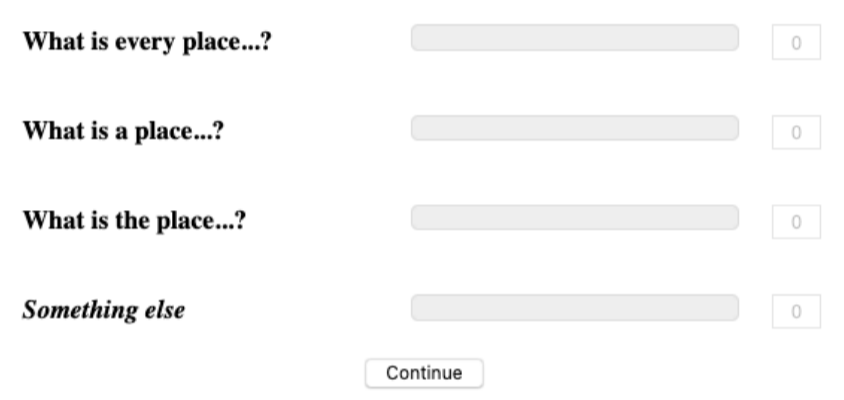
\includegraphics[scale=.52]{figures/sliders_rq.png}
\end{tcolorbox}
% \end{center}
\caption{Example trial in Exp.~1a. \jd{would be neat if this screen shot had the sliders placed at the actual mean values for that item}} %Slider values had to sum to 100, which we rescaled to interpret ratings as a probability distribution reflecting subjective beliefs about intended meaning.}
\label{trial-ex1a}
\end{figure}

The 995 root questions in the database were randomly divided into 32 lists of 30 questions, and 1 list of 35 questions. Within each list, the distribution of \whws and modals was kept roughly proportional to that of the overall set of root questions, so that each participant rated 30 questions which were representative of the overall question distribution in the linguistic features of interest. %reported in Table \ref{rq_dist2}.

In addition, each participant rated 6 control items. Similar to test items, control items were dialogues where an interlocutor asked a question. Rather than a \whq, a polar question was instead asked. These polar questions were created to control for the three paraphrases by containing either an indefinite, definite, or universally quantified noun phrase, similar to the three paraphrases. As such, they are intended to unambiguously convey the meaning encoded in a paraphrase. For example, an \emph{a}-control question like \emph{Can you grab a tissue?} should give rise to highest ratings for the \emph{a}-paraphrase because the speaker explicitly states that they want \emph{a tissue}.
    

Participants first completed four training trials with example dialogues: on two of these, the \emph{a}/\emph{the} paraphrases were best \jd{why both?}, and on the other two the \emph{every} paraphrase was best. We included one modal and one non-modal question for each. Further, on each training trial, participants were instructed to interpret the ellipsis in each paraphrase relative to the content in the target question. For instance, this yields ``What is every place you have skied?" from the displayed ``What is every place\dots?'' in \figref{trial-ex1a}.

\subsubsection{Exclusions and preprocessing}
Questions with higher mean ratings for \emph{something else} than any other option were removed (15\%). These tended to be rhetorical questions (e.g., \emph{Who knows?}, \emph{Who has the time?}, \emph{What are we becoming?}), whose interpretation is orthogonal to the question of whether \emph{wh}-questions are interpreted exhaustively. After exclusions, \jd{XXX} cases remained for analysis. For each item and participant, ratings were normalized such that the three remaining slider values summed to 1.  

\subsubsection{Results}
Because this is a novel task for testing \whq interpretation, we first report a qualitative analysis of the data to assess whether the ratings given for particular items accord with intuitions. We then report the main analysis of interest, which assesses Predictions 1-3 and 5 (all predictions except Goal Sensitivity). 

\begin{figure}[h!]
\centering
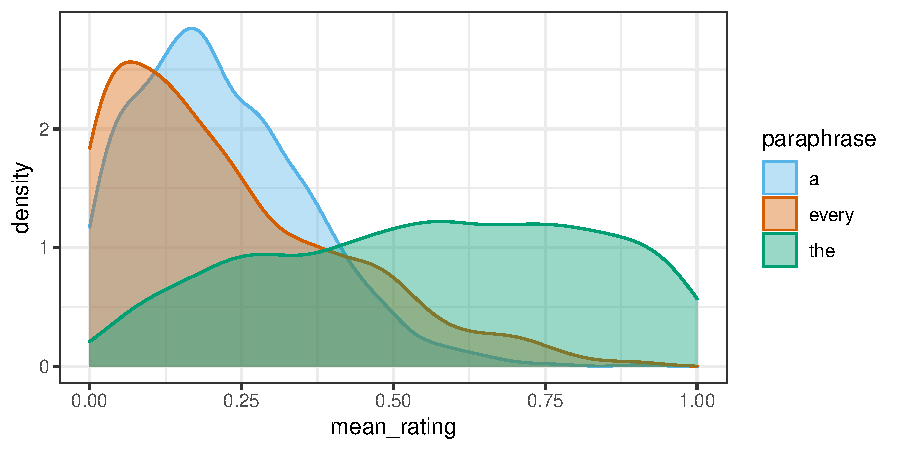
\includegraphics[scale=.8]{figures/ex1a_denisty_mean_ratings.pdf}
\caption{Mean ratings by item in Experiment 1a.}
\label{ex1a_density_mr}
\end{figure}

% \begin{figure}[h!]
% \centering
% 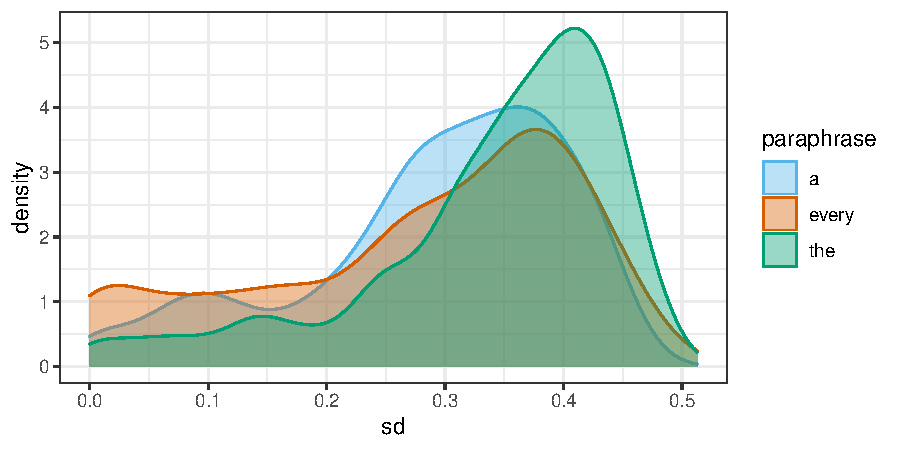
\includegraphics[scale=.8]{figures/ex1a_denisty_sd.pdf}
% \caption{Standard deviations by item in Experiment 1a.\jd{don't need this plot}}
% \label{ex1a_density_sd}
% \end{figure}


\paragraph{Qualitative analysis}

\begin{table}[h!]
    \centering
    \begin{tabular}{|rl|c|c|}
        \hline
        {} & \textbf{Question} & \textbf{Mean} & \textbf{SD} \\
        \hline
        \hline
        (a) & \emph{Where do you live?}       & 1   & 0\\
        (b) & \emph{Where do you work?}       &.99  & .03 \\
        (c) & \emph{What do you drive now?}   &.99    & .0) \\
        (d) & \emph{How do you spell that?}   &.99 &.0\\
        (e) & \emph{When did you first take your first piano lesson?} &.92 & .24 \\
        (f) & \emph{Why are you cutting off the phone?} & .81 & .36\\
        \midrule
        (g) & \emph{What does it have in it?} & .86 & .31 \\
        (h) & \emph{Where have you skied?} &.73 & .37 \\
        \midrule
        (i) & \emph{What is a good brand, a inexpensive?} & .63 & .39\\
        (j) & \emph{What have you seen lately?} & .66 & .3\\
        (k) & \emph{How can I tell you?} & .66 & .42 \\
        (l) & \emph{What else can we talk about?} & .99 & .21\\
        \hline
    \end{tabular}
    \caption{A selection of questions rated highest for each rating. The first group contains questions rated highest on the \emph{the}-paraphrase, the second for the \emph{every}-paraphrase, and the third for the \emph{a}-paraphrase.}
    \label{tab:e1-qualitative}
\end{table}
% \jd{instead of jumping in, say how you chose these items to assess. were they cherry-picked? were they a random sample?}
For each paraphrase, we assesed the questions rated highest for that paraphrase. We refer to \ref{tab:e1-qualitative}. Items (a) - (f) received high \emph{the}-paraphrase ratings (at or near 1). These are all questions that are indeed highly likely to have exactly one answer. 
%  karttunen \& peter 1976; \citeA{srivastav1991}). 
Items (g)-(h) are questions that received high \emph{every} ratings. The first occurred in a context about cooking a casserole; the second in a conversation about the hearer's love for skiing. The exhaustive interpretation---wanting to know all the ingredients in the casserole, wanting to know all the places the hearer has skied---is sensible in both cases.

% all: 102292:4, 61796:21, 87956:4; every: 101503:16, 116314:8, 
Questions that received high \emph{a} ratings often involved recommendations, e.g., (i), which occurred in a discussion about computers where the hearer was an expert. Many questions involved discussions about books or movies, e.g., (j). Other interesting cases included (k), where the speaker struggled to articulate (tell) why they like a certain movie, and (l) where the speaker is struggling to find a conversation topic. In both cases, there are presumably multiple answers (ways to tell, things to talk about), but a single one is sufficient to achieve the speaker's goal.

Overall, the qualitative assessment of individual items suggests that participants understood the task and that the paraphrase ratings are interpretable as proxy judgments for \whq exhaustivity.

\paragraph{Quantitative analysis}

Analyses were conducted on the subset of the \emph{a}/\emph{every} paraphrase data, to assess overall question interpretation bias and the effect of modality and \whw on question interpretation. To this end, we conducted a mixed effects linear regression predicting ratings from fixed effects of \textsc{wh-word} (reference level: \emph{when}), centered measures of whether a modal auxiliary verb was present (\textsc{modalpresent}, before centering: `not present'=0, `present'=1), and \textsc{paraphrase} (before centering: 0 = \emph{every}, 1 = \emph{a}), all 2-way interactions, and the 3-way interaction. The model included the maximal random effects structure justified by the design: random by-item and by-subject intercepts, as well as by-item and by-subject slopes for \textsc{paraphrase}, and by-subject slopes for \textsc{wh} and \textsc{modalpresent}. 

We observed significant 3-way interactions. However, interpreting the interaction terms in this full model is very complex. We thus take the significant three-way interactions as evidence that effects varied by \whw and report the outcome of separate \whw-specific models on each \whw subset of the data: each model included fixed effects of \textsc{paraphrase}, \textsc{modalpresent}, and their interaction, coded as in the full model. 

% EXPERIMENT 1a COEFFICIENT TABLE
\begin{table}[p!]
\begin{center} 
\caption{Coefficient table (predicted $\beta$ coefficient, standard error $SE$, $t$ value, and $p$ value) for \whw-specific models in Exp.~1a. \jd{unify reporting so each beta, se, and t value shows exactly 2 decimal point (ie, insert missing zeroes. also, get rid of vertical lines)}} %Both predictors are dummy-coded and centered (0 is no Modal Present and \emph{every}-paraphrase, 1 for Modal is present and \emph{a}-paraphrase.} 
\label{sub-model_res_ex1a} 
% \vskip .12in
\begin{tabular}{l|lllll} 
\toprule
Wh-Word & {} & $\beta$ & $SE$ & $t$ & $p$\\
\midrule
WHAT & Intercept & .25 & .006 & 38.74 & $<$.0001\\
{} & ModalPresent & .09 & .02 & 4.76 & $<$.0001\\
% \rowcolor{Gainsboro!100}
{} & Paraphrase & -.04 & .01 & -3.13 & $<$.002\\
% \rowcolor{Gainsboro!100}
{} & ModalPresent:Paraphrase & .09 & .03 & 2.8 & $<$.006\\
\bottomrule
\toprule
% HOW & $\beta$ & $SE$ & $t$ & $p$\\
% \midrule
HOW & Intercept & .20 & .01 & 24.63 & $<$.0001\\
{} & ModalPresent & .08 & .02 & 3.62 & $<$ .0005\\
% \rowcolor{Gainsboro!100}
{} & Paraphrase & .06 & .02 & 4.02 & $<$.0001\\
% \rowcolor{Gainsboro!100}
{} & ModalPresent:Paraphrase & .15 & .04 & 3.89 & $<$.0002\\
% \bottomrule
\toprule
% WHERE & $\beta$ & $SE$ & $t$ & $p$\\
% \midrule
WHERE & Intercept & .13 & .01 & 9.35 & $<$.0001\\
{} & ModalPresent & -.03 & .08 & -.37 & .72\\
% \rowcolor{Gainsboro!100}
{} & Paraphrase & -.01 & .02 & -.43 & .6\\
% \rowcolor{Gainsboro!100}
{} & ModalPresent:Paraphrase & .05 & .09 & .52 & .6\\
\bottomrule
\toprule
% {} & WHY & $\beta$ & $SE$ & $t$ & $p$\\
% \midrule
WHY & Intercept & .21 & .01 & 21.57 & $<$.0001\\
{} & ModalPresent & .02 & .02 & .87 & .34\\
% \rowcolor{Gainsboro!100}
{} & Paraphrase & .06 & .02 & 2.71 & $<$.009\\
% \rowcolor{Gainsboro!100}
{} & ModalPresent:Paraphrase & .09 & .05 & 1.82 & .07\\
\bottomrule
\toprule
% WHO & $\beta$ & $SE$ & $t$ & $p$\\
% \midrule
WHO & Intercept & .2 & .03 & 7.6 & $<$.0001\\
{} & ModalPresent & .1 & .06 & 1.6 & .12\\
% \rowcolor{Gainsboro!100}
{} & Paraphrase & .04 & .05 & .79 & .43\\
% \rowcolor{Gainsboro!100}
{} & ModalPresent:Paraphrase & .2 & .11 & 1.71 & .09\\
\bottomrule
\toprule
% WHEN & $\beta$ & $SE$ & $t$ & $p$\\
% \midrule
WHEN & Intercept & .12 & .02 & 6.41 & $<$.0001\\
{} & ModalPresent & .28 & .08 & 3.5 & $<$.004\\
% \rowcolor{Gainsboro!100}
{} & Paraphrase & .15 & .03 & 5.45 & $<$.0001\\
% \rowcolor{Gainsboro!100}
{} & ModalPresent:Paraphrase & .54 & .12 & 4.71 & $<$.0002\\
\bottomrule
\end{tabular} 
\end{center} 
\end{table}






\paragraph{Prediction 1: Is there an overall MA bias?} 
\figref{ex1a_modXwh} \jd{why is this figure made reference to first, if you show us three other plots before it? i'm generally confused by the plot choices, let's discuss} shows mean ratings for each paraphrase. Rather than a preference for MA over MS readings, there was a clear preference for the \emph{the}-paraphrase. There was only a significant MA bias \jd{first say which coefficients you interpret as evidence for MA/MS bias -- perhaps you can merge this in with where you say that the data analysis will only be conducted on the subset of a/every paraphrase ratings} for \emph{what} questions ($\beta$=-0.04, $SE$=0.01, $t$=-3.13, $p<$0.002). In contrast, for \emph{how} ($\beta$=0.06, $SE$=0.02, $t$=4.02, $p<$0.0001), \emph{why} ($\beta$=0.06, $SE$=0.02, $t$=2.71, $p<$0.009) and \emph{when}-questions ($\beta$=0.15, $SE$=0.03, $t$=5.47, $p<$0.0001) there were significant MS biases. Finally, for \emph{where} and \emph{who} there were no significant biases in either direction. 


% \newpage
\begin{figure}[h!]
\centering
\centering
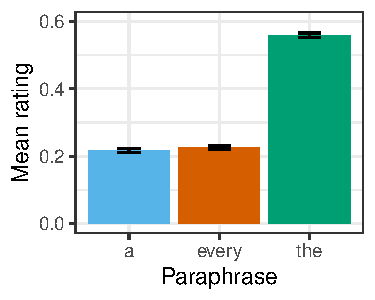
\includegraphics[scale=1]{figures/overall_rq_context.pdf}
\caption{Mean ratings by paraphrase in Experiment 1a. Here and below, error bars indicate 95\% bootstrapped confidence intervals. \jd{include the "something else" ratings in this plot for completeness. add a visualization of variance (eg, plot means as dots with error bars overlaid on violin plots)}}
\label{ex1a_overall}
\end{figure}


\begin{figure}[h!]
\centering
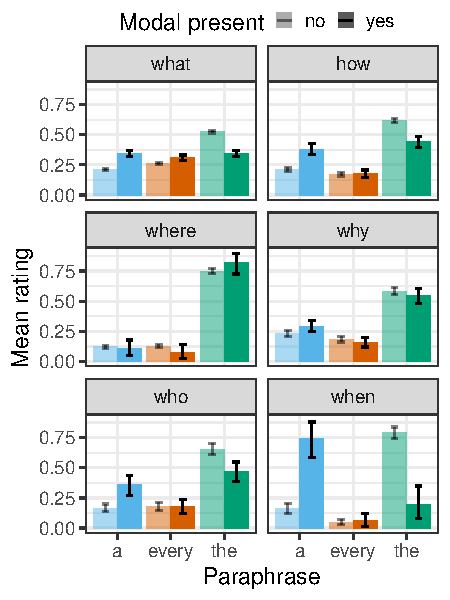
\includegraphics[scale=1]{figures/modxwh_rq_context.pdf}
\caption{Mean ratings by paraphrase, \whw and modality in Experiment 1a. Error bars indicate 95\% bootstrapped confidence intervals.} 
\label{ex1a_modXwh}
\end{figure}


\subsubsection{Predictions 2 and 5: Do modality and \whw modulate question interpretation?} \jd{re-organize this part to fit with the predictions listed in intro?}
Simply, yes. \figref{ex1a_modXwh} presents mean ratings as a function of paraphrase and the presence of a modal, separately for each \whw. We focus the following discussion on the coefficients and $p$-values in the \tableref{sub-model_res_ex1a}.

For \emph{what} questions, the overall MA bias is inverted to an MS bias when a modal is present. \jd{provide two examples that show the contrast?}%(note the significant positive shift in coefficient values when a modal is present).

\emph{How}, \emph{why}, and \emph{when} pattern together in showing an overall MS bias, confirming previously made predictions \cite{ginzburg1995,asherlascarides1998}. \emph{Who} and \emph{where} show no overall bias, but \emph{who} shows a preference for MS while \emph{where} for MA, in contrast to those predictions. \jd{this last sentence is unparseable}


Thus, the prediction that \emph{who} is biased for MA is not confirmed. Only \emph{what} displayed an MA bias. Qualitative inspection of those questions which received the highest \emph{every} ratings revealed that some of these were questions with a plural-marked complex \emph{wh}-phrase (e.g., \emph{What cities are they looking at}, .92, .15) that slipped through our initial filters. These were intended to be excluded precisely because they are expected to not be ambiguous between MS and MA. \jd{again, this makes it sound like we're just trying to ecxlude cases that don't work in our favor. explain why that's not the case} However, future work should explicitly include and test complex \emph{wh}-questions. If they really are unambiguous, then plural-marked complex questions should show a clear preference for \emph{every}, and singular-marked ones for \emph{a} (or \emph{the}).

The presence of a modal yielded higher MS ratings for \emph{what}, \emph{how}, and \emph{when} questions, while this increase was only marginally significant for  \emph{why} and \emph{who} questions, and did not reach significance for \emph{where} questions. \jd{i'm confused -- why are the interactions not reported, even though they're doing the main work?} 

%In general, the presence of a modal auxiliary shifts probability away from \emph{the}-paraphrases, and redistributes it to \emph{a}-paraphrases: in \figref{ex1a_modXwh} this can be seen in the higher orange than blue \emph{a} bars accompanied by the lower orange than blue \emph{the} bars, while the changes to \emph{every} are negligible. 

Overall, these results confirm the observation that modal auxiliaries facilitate MS readings. 

%%%%%%%%%%%%%%%%%%%%%%%%%%%%%%%%%%%%%%%%%%%%%%%%%
\subsection{Experiment 1b: embedded question interpretation}
%%%%%%%%%%%%%%%%%%%%%%%%%%%%%%%%%%%%%%%%%%%%%%%%%

Exp.~1b tested exhaustivity of questions embedded under a variety of predicates, some of which have been claimed to semantically condition exhaustivity \jd{cite}.

\jd{edit this whole section so the methods and results sections mirror the re-organization of exp 1a}

\subsubsection{Method}

\paragraph{Participants}
On Prolific, we recruited \mm{1073--is this right?} speakers who were paid about \$14/hr for their work. Eligible participants had to be born and currently reside in the US, as well as speak English as their first language. We included an addition question at the end of the study about native languages, and excluded 25 participants who reported native languages other than English. We additionally removed 37 participants for failing 2 out of 6 control trials.

\paragraph{Procedure and materials}
The procedure and materials were nearly identical to that of Experiment 1a, except in two respects. Figure \figref{trial-ex1b}.

First, the materials were embedded questions from the Switchboard corpus rather than root question. The 1075 embedded question database was divided into 35 lists of 30 questions, and 1 list of 35 questions. The distribution of \whws and modals was kept roughly proportional to the overall distribution.

Second, and in virtue of the first difference, the task itself changed in two ways. First, participants responded to the question, \emph{Based on the question in red, how likely do you think it is the that speaker means each of the following?}. Second, the paraphrases included ellipses before the \whw as well, to indicate that the paraphrase involved the lingusitic content occuring prior to the \whw.

\begin{figure}%[H]
% \begin{center}
\begin{tcolorbox}[colback=white]

\textbf{Speaker $\#$2}: \\
\textbf{Speaker $\#$1}: um.\\
\textbf{Speaker $\#$2}: so. well, uh, did you hear about that killeen massacre or whatever?\\
\textbf{Speaker $\#$1}: yeah, the, did it happen at a cafeteria or something?\\
\textbf{Speaker $\#$2}: yeah, right. that kind of i mean it just makes \color{red}you wonder \textbf{how people get guns}\color{black}\\

\noindent \emph{Based on the sentence in red, how likely do you think it is that the speaker means each of the following?}\\

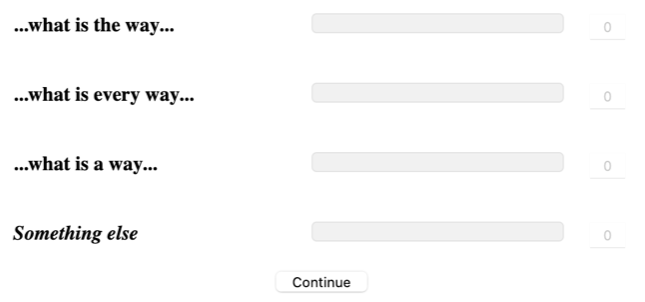
\includegraphics[scale=.5]{figures/sliders_eq.png}
\end{tcolorbox}
% \end{center}
\caption{Example trial in Exp.~1b.}
\label{trial-ex1b}
\end{figure}

\subsubsection{Exclusions and preprocessing}
\mm{what is the equivalent of a rhetorical question in embedded cases?}
Questions that received higher ratings for \emph{something else} than any other option were removed (15.5\%). These are questions like 
``but they do read. uh, where a lot of people don't have any interest in it at all,'' 
``they're real liberal now and to where probably fifty or a hundred years ago, um, the democrat party being liberal like they are?,'' 
``but i like that where they run tense,'' 
whose interpretation is orthogonal to the question of whether \emph{wh}-questions are interpreted exhaustively. \jd{um, it's not just an issue of the question of exhaustivity being orthogonal, it's also that these clearly include cases that shouldn't have been included in the first place. also, these aren't readable if they just occur one after the other. put in between quotes instead of italicizing and be explicit about the issue with the sentences.} After exclusion, ratings were normalized such that for each participant and item, the three remaining slider values summed to 1.  

\subsubsection{Qualitative analysis}
Because this is a novel task for testing \whq interpretation, we begin by qualitatively assessing whether the ratings given for particular items accord with intuitions about the best paraphrase.

Questions like 
``I know who you’re talking about,'' (.94,.13), 
``Do you know who the guy was that was playing the wagon driver?'' (.95,.14), 
``My mother taught me how to make it,'' (.93,.2), and
``I forget how she got it,'' (.86,.14) 
all received high mean ratings for \emph{the}-paraphrase. For these questions, it is again possible but unlikely that there is more than one answer.

Questions that received a high rating for the \emph{every}-paraphrase included 
``So He knew who worked there,'' (.79,.35), 
``I have got to be so much more careful with what I do,'' (.77,.35), 
% \emph{And then we have a local rag here in town that I pick up periodically and read just to see what's going on in our little community.} (.77,.34), and
``Nobody can predict what's going to happen in twenty years,'' (.69,.38).
In the first case, the preceeding discourse context included an explicit domain restriction (\emph{there's only a few people that worked there}), making an MA reading possible. The second question occurs in a context about an injury, where the necessissity for caution requires MA. Finally, the third question occurs in the context of planning for possible events so an \emph{every} reading is salient.

Questions that received a high rating for the \emph{a}-paraphrase included
``I’m not real sure why anybody would need a full automatic weapon,'' (.61,.4), 
``I don’t know how to make it better for them,'' (.57,.4), and 
``I don’t know when I’m going to get them all,'' (.49,.4). In all these three cases, an MS interpretation is sufficient to achieve the speaker's goal.

Overall, the qualitative assessment of individual items suggests that participants understood the task and that the ratings are interpretable.




\subsubsection{Data analysis}
Analyses were conducted to assess overall question interpretation bias and the effect of modality and \whw on question interpretation. To this end, we conducted a mixed effects linear regression predicting rating from fixed effects of \textsc{paraphrase} (reference level: \emph{every}), \textsc{wh-word} (reference level: \emph{when}), a dummy-coded and mean-centered measure of whether a modal auxiliary verb was present (\textsc{modalpresent}), all 2-way interactions between fixed effects, and the 3-way interaction. We included the maximal random effects structure justified by the design: random by-item and by-subject intercepts, as well as by-item and by-subject slopes for \textsc{paraphrase}, and by-subject slopes for \textsc{wh} and \textsc{modalpresent}. 

We observed significant 3-way interactions. %(Wh.how x ModalPresent (MP) x Paraphrase.a (Para): $\beta$=-.45, $SE$=.2, $t$=-2.2, $p<$.05; Wh.where x MP x Para.a: $\beta$=-.51, $SE$=.23, $t$=-2.2, $p<$.05; Wh.why x MP x Para.a: $\beta$=-.47, $SE$=.21, $t$=-2.2, $p<$.05). 
However, interpreting the interaction terms in this full model is very complex because two of our predictors include $>$ 3 levels. We thus take the significant three-way interactions as evidence that effects varied by \whw and  report the outcome of separate specific models on each \whw subset of the data: each model included fixed effects of \textsc{paraphrase}, \textsc{modalpresent}, and their interaction, coded as in the full model. 

An exhaustive MA bias is evidenced as a significantly negative coefficient of the `a vs.~every' \textsc{paraphrase} contrast; a non-exhaustive MS bias as a significantly positive coefficient. An introduction or strengthening of an MS bias in the presence of a modal is evidenced in a significantly positive interaction of \textsc{modalpresent} with the `a vs.~every' \textsc{paraphrase} contrast. The results of each model are shown in \tableref{sub-model_res_ex1b}, with the two relevant contrasts highlighted in gray.

% EXPERIMENT 1b COEFFICIENT TABLE
\begin{table}[p!]
\begin{center} 
\caption{Coefficient table (predicted $\beta$ coefficient, standard error $SE$, $t$ value, and $p$ value) for \whw-specific models in Experiment 1b. Both predictors are dummy-coded and centered (0 is no Modal Present and \emph{every}-paraphrase, 1 for Modal is present and \emph{a}-paraphrase.} 
\label{sub-model_res_ex1b} 
% \vskip .12in
\begin{tabular}{l|lllll} 
\toprule
Wh-Word & {} & $\beta$ & $SE$ & $t$ & $p$\\
\midrule
WHAT & Intercept & .26 & .01 & 22.85 & $<$.0001\\
{} & ModalPresent & .07 & .01 & 5.83 & $<$.0001\\
% \rowcolor{Gainsboro!100}
{} & Paraphrase & -.12 & .02 & -6.51 & $<$.0001\\
% \rowcolor{Gainsboro!100}
{} & ModalPresent:Paraphrase & .09 & .03 & 2.77 & $<$.006\\
\midrule
% HOW & $\beta$ & $SE$ & $t$ & $p$\\
% \midrule
HOW & Intercept & .22 & .01 & 19.21 & $<$.0001\\
{} & ModalPresent & .03 & .01 & 2.37 & $<$.02\\
% \rowcolor{Gainsboro!100}
{} & Paraphrase & .06 & .01 & 3.99 & $<$.0002\\
% \rowcolor{Gainsboro!100}
{} & ModalPresent:Paraphrase & 0.09 & .02 & 4.12 & $<$.0001\\
% \bottomrule
\midrule
% WHERE & $\beta$ & $SE$ & $t$ & $p$\\
% \midrule
WHERE & Intercept & .21 & .02 & 13.69 & $<$.0001\\
{} & ModalPresent & 0.03 & 0.03 & 1.09 & .28\\
% \rowcolor{Gainsboro!100}
{} & Paraphrase & .01 & .03 & .22 & .83\\
% \rowcolor{Gainsboro!100}
{} & ModalPresent:Paraphrase & .2 & .08 & 2.42 & $<$0.02\\
\midrule
% {} & WHY & $\beta$ & $SE$ & $t$ & $p$\\
% \midrule
WHY & Intercept & .19 & .01 & 27.9 & $<$.0001\\
{} & ModalPresent & 0.07 & .02 & 4.06 & $<$.0002\\
% \rowcolor{Gainsboro!100}
{} & Paraphrase & .05 & .02 & 2.42 & $<$.05\\
% \rowcolor{Gainsboro!100}
{} & ModalPresent:Paraphrase & .1 & .04 & 2.51 & $<$.02\\
\midrule
% WHO & $\beta$ & $SE$ & $t$ & $p$\\
% \midrule
WHO & Intercept & .25 & .02 & 12.08 & $<$.0001\\
{} & ModalPresent & .08 & .07 & 1.15 & .26\\
% \rowcolor{Gainsboro!100}
{} & Paraphrase & -.05 & .06 & -.82 & .42\\
% \rowcolor{Gainsboro!100}
{} & ModalPresent:Paraphrase & -.01 & .14 & -.04 & .99\\
\midrule
% WHEN & $\beta$ & $SE$ & $t$ & $p$\\
% \midrule
WHEN & Intercept & .23 & .04 & 6.37 & $<$.0001\\
{} & ModalPresent & .03 & .06 & .51 & .62\\
% \rowcolor{Gainsboro!100}
{} & Paraphrase & .12 & .06 & 2.05 & .07\\
% \rowcolor{Gainsboro!100}
{} & ModalPresent:Paraphrase & .14 & .14 & 1.05 & .31\\
\bottomrule
\end{tabular} 
\end{center} 
\end{table}

\subsubsection{Results}

\begin{figure}[h!]
\centering
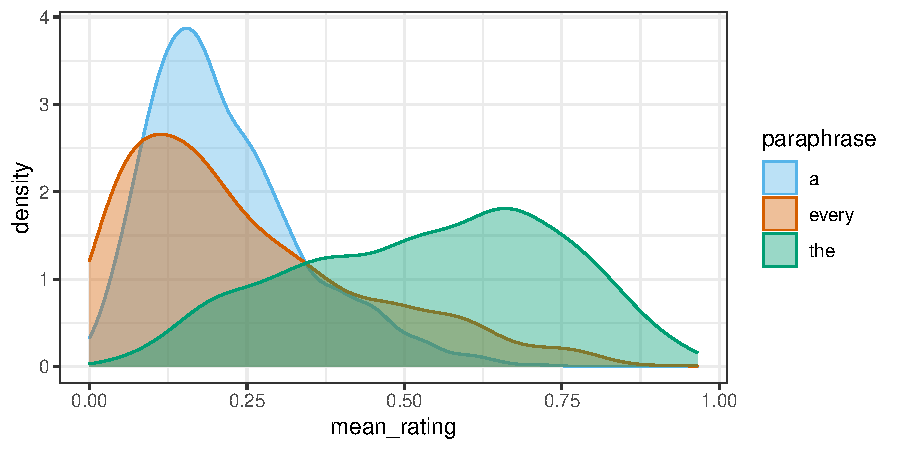
\includegraphics[scale=1]{figures/ex1b_denisty_mean_ratings.pdf}
\caption{Mean ratings by item for \emph{a}- and \emph{every}-paraphrases in Experiment 1b.}
\label{ex1b_density_mr}
\end{figure}

\begin{figure}[h!]
\centering
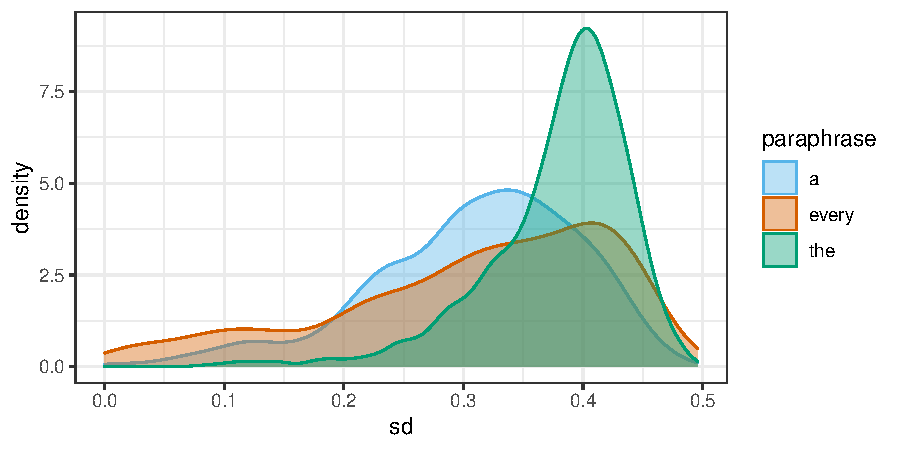
\includegraphics[scale=1]{figures/ex1b_denisty_sd.pdf}
\caption{SD by item for \emph{a}- and \emph{every}-paraphrases in Experiment 1b.}
\label{ex1b_density_sd}
\end{figure}

\begin{figure}[h!]
% \begin{subfigure}[b]{\columnwidth}
\centering
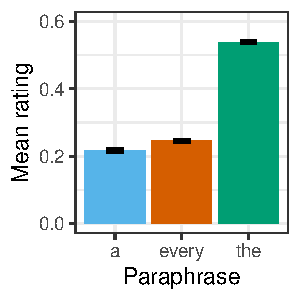
\includegraphics[scale=1]{figures/overall_eq_context.pdf}
\caption{Mean ratings by paraphrase in Experiment 1b. Here and below, error bars indicate 95\% bootstrapped confidence intervals.}
\label{ex1b_overall}
\end{figure}


\paragraph{Prediction 1: Is there an overall MA bias?}
\figref{ex1b_overall} plots mean rating as a function of Paraphrase. We found evidence for a significant MA bias with \emph{what}-questions ($\beta$=-.12, $SE$=.02, $t$=-6.51, $p<$0.0001), and a non-significant preference for MA with \emph{who}-questions ($\beta$=-.05, $SE$=.06, $t$=-.82, $p$=.99). The remaining \whqs revealed either significant bias (\emph{how}: $\beta$=.06, $SE$=.01, $t$=3.99, $p<$0.0002; \emph{why}: $\beta$=.05, $SE$=.02, $t$=2.42, $p<$0.05) or preference (\emph{where}: $\beta$=.01, $SE$=.03, $t$=.22, $p$=.83; \emph{when}: $\beta$=.12, $SE$=.06, $t$=2.05, $p<$0.07) for MS. 

\begin{figure}[h!]
\centering
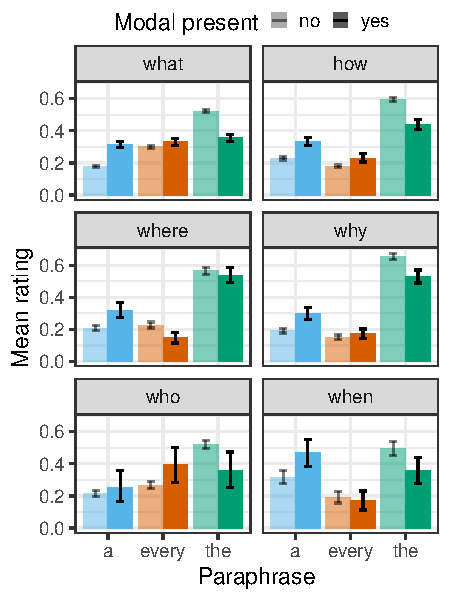
\includegraphics[scale=1]{figures/modxwh_eq_context.pdf}
\caption{Mean ratings by paraphrase, \whw and modality in Experiment 1b. Error bars indicate 95\% bootstrapped confidence intervals.} 
\label{ex1b_modXwh}
\end{figure}

\paragraph{Predictions 2,3 and 5: Is MS interpretation modulated by the presence of modality, by matrix verb, and by \whw?}
Yes. \figref{ex1b_modXwh} plots mean rating as a function of ModalPresent, Wh-Word and Paraphrase. Interestingly, the presence of a modal significantly reversed the initial MA bias for \emph{what}- questions ($\beta$=0.09, $SE$=0.03, $t$=2.77, $p<$0.006), but only attenuated the MA preference in \emph{who}-questions. The remaining \whqs patterned together, the presence of a modal strengthened the MS bias significantly (except for \emph{when}-questions, where the effect did not reach significance).

\figref{ex1b_matrix_verbs} presents several matrix verbs that are of theoretical interest. Unfortunately, we encounter a sparse data problem for most of these verbs so we focus on \emph{know}. \figref{ex1b_modXwh_know} plots mean rating as a function of Paraphrase, Wh-Word and Modality. We found significant 2-way interactions between Wh-Word and Paraphrase in \emph{know-wh}: a significant MA bias for \emph{know-what} ($\beta$=-.09, $SE$=0.02, $t$=-4.75, $p<$0.0001) and a non-significant MA preference for \emph{know-who} ($\beta$=-.1, $SE$=0.06, $t$=-1.77, $p$=0.09), while a signfifcant MS bias for \emph{know-how} ($\beta$=.08, $SE$=.02, $t$=4.12, $p<$0.0001) and \emph{know-when} ($\beta$=0.22, $SE$=0.09, $t$=2.41, $p<$0.05), and non-significant MS preference for \emph{know-where}, \emph{know-why}.

The addition of a modal either reversed an MA bias (\emph{what}: $\beta$=0.12, $SE$=0.04, $t$=2.74, $p<$0.007) or strengthed the MS bias (\emph{know}: $\beta$=0.01, $SE$=0.03, $t$=2.93, $p<$0.005, \emph{where}: $\beta$=0.26, $SE$=0.01, $t$=2.58, $p<$0.03, \emph{why}: $\beta$=0.19, $SE$=0.07, $t$=2.49, $p<$0.02). However, there was no effect of modal for \emph{know-who}, \emph{know-when} questions.

\begin{figure}[h!]
\centering
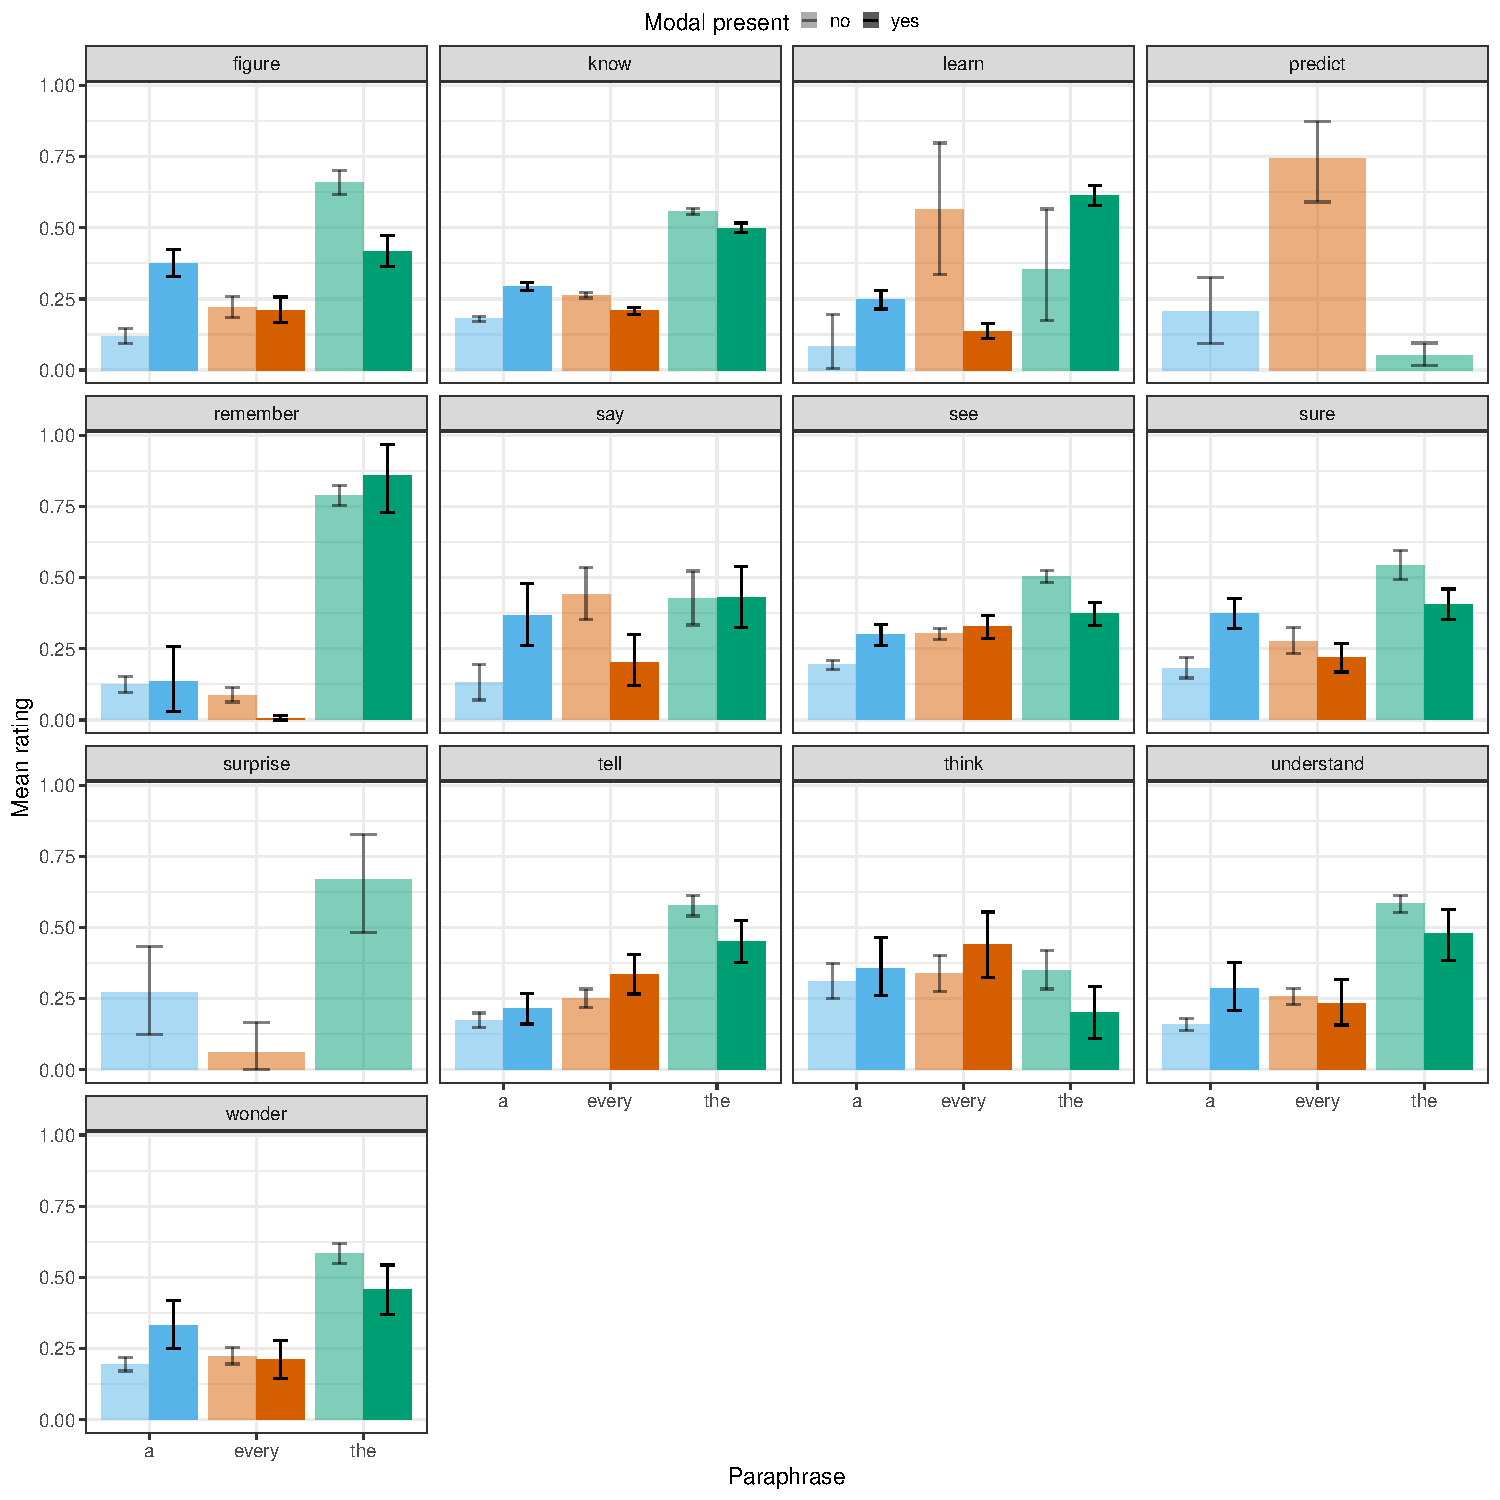
\includegraphics[scale=.6]{figures/matrixverbs_threotical_context.pdf}
\caption{Mean ratings by paraphrase for several Matrix Verbs that have been of interest in the theoretical literature, in Experiment 1b. Error bars indicate 95\% bootstrapped confidence intervals.} 
\label{ex1b_matrix_verbs}
\end{figure}


\begin{figure}[h!]
\centering
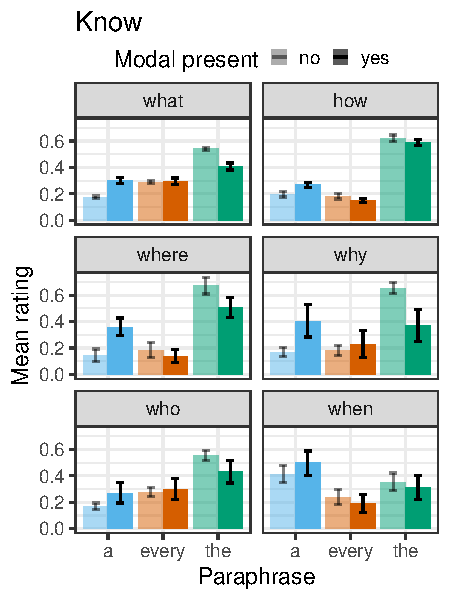
\includegraphics[scale=1]{figures/modwh_know_context.pdf}
\caption{Mean ratings by paraphrase, \whw and modality for questions embedded under \emph{know} in Experiment 1b. Error bars indicate 95\% bootstrapped confidence intervals.} 
\label{ex1b_modXwh_know}
\end{figure}

\subsection{Discussion}

Given our results, we conclude that indeed the MS reading of \emph{wh}-questions is modulated by various linguistic factors. Figure \figref{exs1_density} plots the distribution of mean ratings by item and by linguistic factors. As is clear from the plots, there is immese variation in interpretation.

\begin{figure}[h!]
\centering
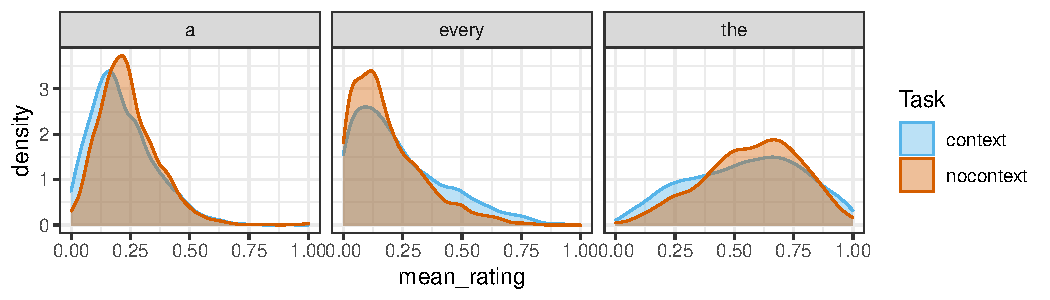
\includegraphics[scale=1]{figures/denisty_context_ratings.pdf}
\caption{Mean ratings by item for \emph{a}- and \emph{every}-paraphrases, across Experiments 1a and 1b.} 
\label{exs1_density}
\end{figure}


% \begin{figure}[h!]
% \centering
% 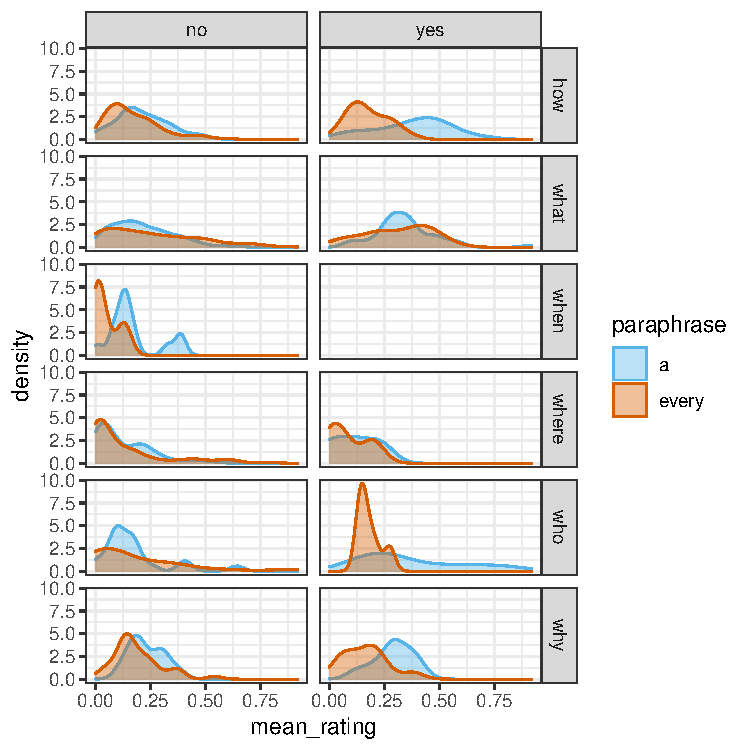
\includegraphics[scale=1]{figures/denisty_mean_ratings_factors.pdf}
% \caption{Mean ratings by item for \emph{a}- and \emph{every}-paraphrases, across Experiments 1a and 1b.} 
% \label{exs1_factors_density}
% \end{figure}

The most robust finding is that the presence of a modal significantly increases ratings for MS than the absence. This effect held even though we grouped both necessity and possibility modals together. Looking more deeply at the distribution of readings with particular modals, \mm{add some discussion about modality here, possibility versus necessisity}



There were some slight differences between the two experiments. While there was no overall MA bias for root questions, there was more of a bias in embedded questions. In both cases, however, ratings were significantly modulated by the Wh-word and the presence of modality. 


\mm{were the differences in the two experiments driven by know-wh? like, can we attribute the preference for MA in experiment 1b to know-wh? How would we test that? Can we test a model on the 1b data making a dummy coded variable for know-wh versus everything else?}


% \mm{conclusion: MS modulated by various LF factors...maybe brief discussion of sematnics theories. We also see no overall MA bias....want to show that there's lots variability in interpretation with HISTOGRAMS OF THE EVERY AND THE A REATINGS MEAN-BY-ITEM}










%%%%%%%%%%%%%%%%%%%%%%%%%%%%%%%%%%%%%%%%%%%%%%%%%
%%%%%%%%%%%%%%%%%%%%%%%%%%%%%%%%%%%%%%%%%%%%%%%%%
% EXPERIMENTS WITHOUT CONTEXT
%%%%%%%%%%%%%%%%%%%%%%%%%%%%%%%%%%%%%%%%%%%%%%%%%
%%%%%%%%%%%%%%%%%%%%%%%%%%%%%%%%%%%%%%%%%%%%%%%%%

\section{Experiments without context}
We've shown that there is no MA bias, but that linguistic factors like both the Wh-word and Modality can influence the distribution of interpretiatons. It's possible that, by removing the contexts of utterance we understand the extent to which \whq interpretation changes. In this second set of experiments, we conducted the same experiment with root and embedded questions above, however without the ten preceding lines of discourse.

\subsection{Predictions}

Based on observations from the literature, we expect (1) questions to be overall biased for MA, (2) Modal questions to be biased for MS, and possibly non-modal questions for MA, (3) \emph{who}-questions to be biased for MA, and others for MS. For experiment 1b with embedded questions, we predict that \emph{know-wh} will be biased for MA, but also that there may be some interactions with \whw.

Besides the predictions about overal and specific biases, we might expect differences between the Context and NoContext experiments if the discourse context provides crucial information relevant to determining the interpretation of root and embedded questions, which are underspecified for (non)-exhaustivity.

%%%%%%%%%%%%%%%%%%%%%%%%%%%%%%%%%%%%%%%%%%%%%%%%%
\subsection{Experiment 2a: Root questions without context}
%%%%%%%%%%%%%%%%%%%%%%%%%%%%%%%%%%%%%%%%%%%%%%%%%


\subsubsection{Method}

\paragraph{Participants}
656 participants, 25 removed for non-native. 51 additional participants were removed for failing controls.

\paragraph{Procedure and materials}
The procedure and materials were nearly identical to that of Experiment 1a as presented in \figref{trial-ex1a}, except participants were shown the root questions without the ten preceeding lines of discourse.


\subsubsection{Exclusions and preprocessing}
Questions that received higher ratings for \emph{something else} than any other option were removed (16.3\%). After exclusion, ratings were normalized such that for each participant and item, the three remaining slider values summed to 1.

\subsubsection{Data analysis}
Analyses were conducted to assess overall question interpretation bias and the effect of modality and \whw on question interpretation. To this end, we conducted a mixed effects linear regression predicting critical ratings from fixed effects of \textsc{wh-word} (reference level: \emph{when}), dummy-coded and mean-centered measures of whether a modal auxiliary verb was present (\textsc{modalpresent}, 0 = not present, 1 = present) and \textsc{paraphrase} (0 = \emph{every}, 1 = \emph{a}), all 2-way interactions between fixed effects, and the 3-way interaction. We included the maximal random effects structure justified by the design: random by-item and by-subject intercepts, as well as by-item and by-subject slopes for \textsc{paraphrase}, and by-subject slopes for \textsc{wh} and \textsc{modalpresent}. 



% EXPERIMENT 2a COEFFICIENT TABLE
\begin{table}
\begin{center} 
\caption{Coefficient table (predicted $\beta$ coefficient, standard error $SE$, $t$ value, and $p$ value) for \whw-specific models in Experiment 2a. Both predictors are dummy-coded and centered (0 is no Modal Present and \emph{every}-paraphrase, 1 for Modal is present and \emph{a}-paraphrase.} 
\label{sub-model_res_ex2a} 
% \vskip .12in
\begin{tabular}{l|lllll} 
\toprule
Wh-Word & {} & $\beta$ & $SE$ & $t$ & $p$\\
\midrule
WHAT & Intercept & .23 & .005 & 44.12 & $<$.0001\\
{} & ModalPresent & .08 & .01 & 5.43 & $<$.0001\\
% \rowcolor{Gainsboro!100}
{} & Paraphrase & .02 & .01 & 1.4 & .16\\
% \rowcolor{Gainsboro!100}
{} & ModalPresent:Paraphrase & .02 & .02 & .81 & .42\\
% \bottomrule
\midrule
% HOW & $\beta$ & $SE$ & $t$ & $p$\\
% \midrule
HOW & Intercept & .19 & .01 & 29.07 & $<$.0001\\
{} & ModalPresent & .05 & .02 & 2.79 & $<$.006\\
% \rowcolor{Gainsboro!100}
{} & Paraphrase & .09 & .01 & 6.27 & $<$.0001\\
% \rowcolor{Gainsboro!100}
{} & ModalPresent:Paraphrase & .07 & .03 & 2.64 & $<$.001\\
% \bottomrule
\midrule
% WHERE & $\beta$ & $SE$ & $t$ & $p$\\
% \midrule
WHERE & Intercept & .13 & .01 & 13.52 & $<$.0001\\
{} & ModalPresent & -.01 & .04 & -.19 & .85\\
% \rowcolor{Gainsboro!100}
{} & Paraphrase & .06 & .01 & 5.04 & $<$.0001\\
% \rowcolor{Gainsboro!100}
{} & ModalPresent:Paraphrase & -.1 & .06 & -1.64 & .1\\
% \bottomrule
\midrule
% {} & WHY & $\beta$ & $SE$ & $t$ & $p$\\
% \midrule
WHY & Intercept & .2 & .01 & 24.32 & $<$.0001\\
{} & ModalPresent & .03 & .02 & 1.8 & $<$.08\\
% \rowcolor{Gainsboro!100}
{} & Paraphrase & .08 & .02 & 4.78 & $<$.0001\\
% \rowcolor{Gainsboro!100}
{} & ModalPresent:Paraphrase & .06 & .04 & 1.77 & $<$.09\\
% \bottomrule
\midrule
% WHO & $\beta$ & $SE$ & $t$ & $p$\\
% \midrule
WHO & Intercept & .21 & .02 & 10.46 & $<$.0001\\
{} & ModalPresent & .03 & .05 & .62 & .54\\
% \rowcolor{Gainsboro!100}
{} & Paraphrase & .03 & .03 & 1.05 & .3\\
% \rowcolor{Gainsboro!100}
{} & ModalPresent:Paraphrase & .2 & .08 & 2.29 & $<$.03\\
% \bottomrule
\midrule
% WHEN & $\beta$ & $SE$ & $t$ & $p$\\
% \midrule
WHEN & Intercept & .11 & .02 & 5.99 & $<$.0001\\
{} & ModalPresent & .17 & .06 & 2.71 & $<$.02\\
% \rowcolor{Gainsboro!100}
{} & Paraphrase & .13 & .03 & 3.73 & $<$.003\\
% \rowcolor{Gainsboro!100}
{} & ModalPresent:Paraphrase & .04 & .12 & .29 & .77\\
\bottomrule
\end{tabular} 
\end{center} 
\end{table}



\subsubsection{Results}

\begin{figure}[h!]
\centering
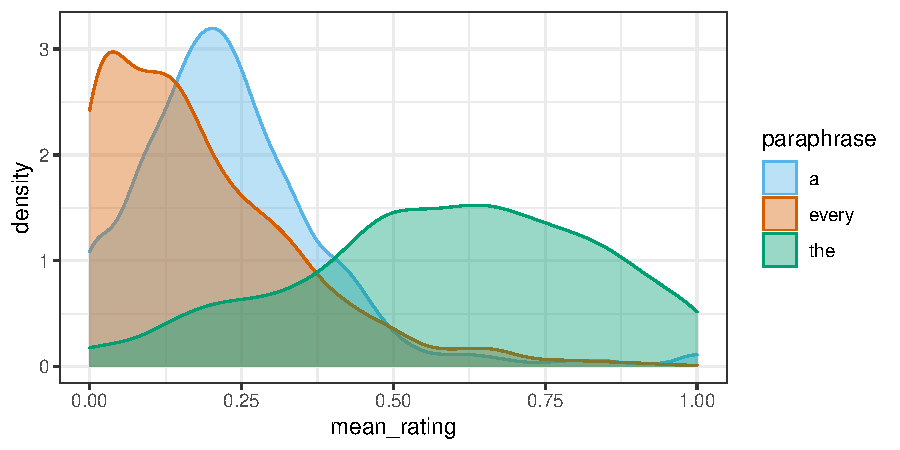
\includegraphics[scale=1]{figures/ex2a_denisty_mean_ratings.pdf}
\caption{Mean ratings by item for \emph{a}- and \emph{every}-paraphrases in Experiment 2a.}
\label{ex2a_density_mr}
\end{figure}

% \begin{figure}[h!]
% \centering
% 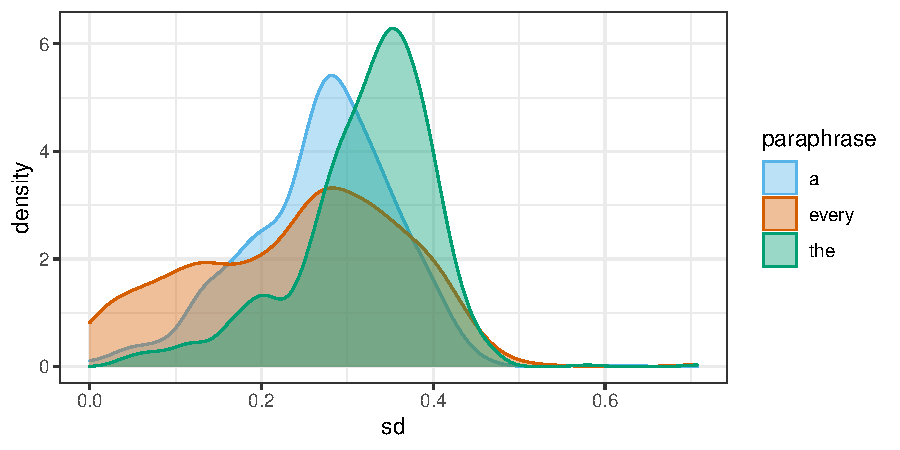
\includegraphics[scale=1]{figures/ex2a_denisty_sd.pdf}
% \caption{Mean ratings by item for \emph{a}- and \emph{every}-paraphrases in Experiment 2a.}
% \label{ex2a_density_sd}
% \end{figure}

\paragraph{Prediction 1: Is there an overall MA bias?}

Figure \figref{ex2a_overall} plots the overal mean ratings for the three paraphrases. There were no significant biases for MA for any \whq. \emph{How}, \emph{where}, \emph{why}, \emph{when} patterned together in showing significant MS biases, while \emph{what} and \emph{who} patterned together in having positive (but not significant) coefficiants, revealing a preference towards an MS bias.
\begin{figure}[h!]
\centering
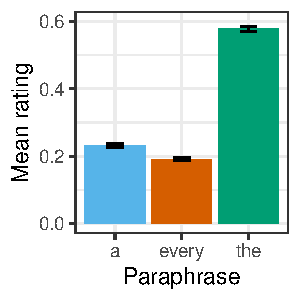
\includegraphics[scale=1]{figures/overall_nocontext_root.pdf}
\caption{Mean ratings by paraphrase in Experiment 2a. Here and below, error bars indicate 95\% bootstrapped confidence intervals.}
\label{ex2a_overall}
\end{figure}


\paragraph{Predictions 2 and 5: Is MS modulated by the presence of modality and \whw?}
\figref{ex2a_modXwh} plots mean rating as a function of ModalPresent, Wh-Word and Paraphrase. As just discussed, there were some significant differences in initial biases for MS vs. MA based on the different \whqs: \emph{how}, \emph{where}, \emph{why}, \emph{when} showed a significant MS bias, while \emph{what} and \emph{who} did not (though were positively skewed towards MS). This finding is different from the previous two studies, where at least \emph{what} and \emph{who} showed MA biases.

Given that there were no \whqs biased for MA, the presence of a modal did not significantly reverse any biases, although for \emph{when} and \emph{where} the modal appeared to neutralize the MS bias. For \emph{how}, \emph{why} and \emph{who} the interaction with modality was significant (and positively skewed towards MS), but not significant for \emph{when}.


\begin{figure}[h!]
\centering
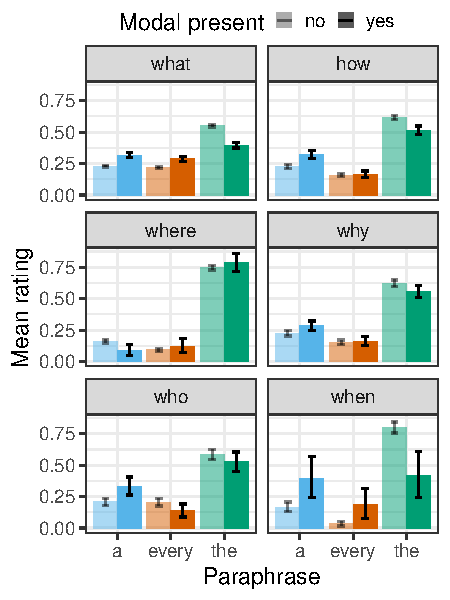
\includegraphics[scale=1]{figures/modxwh_nocontext_root.pdf}
\caption{Mean ratings by paraphrase, \whw and modality in Experiment 2a. Error bars indicate 95\% bootstrapped confidence intervals.} 
\label{ex2a_modXwh}
\end{figure}







%%%%%%%%%%%%%%%%%%%%%%%%%%%%%%%%%%%%%%%%%%%%%%%%% 
% EXPERIMENT 2b
%%%%%%%%%%%%%%%%%%%%%%%%%%%%%%%%%%%%%%%%%%%%%%%%%
\subsection{Experiment 2b: Embedded questions without context}

\subsubsection{Method}

\paragraph{Participants}
717 participants, 28 removed for non-native, 43 removed for failing controls.

\paragraph{Procedure and materials}
The procedure and materials were nearly identical to that of Experiment 2b as presented in \figref{trial-ex1b}, except--as with Experiment 2a, participants were not shown the 10 preceeding lines of discourse.


\subsubsection{Exclusions and preprocessing}
Questions that received higher ratings for \emph{something else} than any other option were removed (17.8\%). After exclusion, ratings were normalized such that for each participant and item, the three remaining slider values summed to 1.

% \subsubsection{Qualitative analysis}
% Because this is a novel task for testing \whq interpretation, we begin by qualitatively assessing whether the ratings given for particular items accord with intuitions about the best paraphrase.

\subsubsection{Data analysis}
Analyses were conducted to assess overall question interpretation bias and the effect of modality and \whw on question interpretation. To this end, we conducted a mixed effects linear regression predicting critical ratings from fixed effects of \textsc{wh-word} (reference level: \emph{when}), dummy-coded and mean-centered measures of whether a modal auxiliary verb was present (\textsc{modalpresent}, 0 = not present, 1 = present) and \textsc{paraphrase} (0 = \emph{every}, 1 = \emph{a}), all 2-way interactions between fixed effects, and the 3-way interaction. We included the maximal random effects structure justified by the design: random by-item and by-subject intercepts, as well as by-item and by-subject slopes for \textsc{paraphrase}, and by-subject slopes for \textsc{wh} and \textsc{modalpresent}. 


% EXPERIMENT 2b COEFFICIENT TABLE
\begin{table}
\begin{center} 
\caption{Coefficient table (predicted $\beta$ coefficient, standard error $SE$, $t$ value, and $p$ value) for \whw-specific models in Experiment 2b. Both predictors are dummy-coded and centered (0 is no Modal Present and \emph{every}-paraphrase, 1 for Modal is present and \emph{a}-paraphrase.} 
\label{sub-model_res_ex2b} 
% \vskip .12in
\begin{tabular}{l|lllll} 
\toprule
Wh-Word & {} & $\beta$ & $SE$ & $t$ & $p$\\
\midrule
WHAT & Intercept & .24 & .01 & 21.89 & $<$.0001\\
{} & ModalPresent & .07 & .01 & 5.76 & $<$.0001\\
% \rowcolor{Gainsboro!100}
{} & Paraphrase & -.004 & .02 & -.2 & .85\\
% \rowcolor{Gainsboro!100}
{} & ModalPresent:ModalPresent & .06 & .03 & 2.5 & $<$.02\\
\midrule
% HOW & $\beta$ & $SE$ & $t$ & $p$\\
% \midrule
HOW & Intercept & .02 & .01 & 23.86 & $<$.0001\\
{} & ModalPresent & .04 & .01 & 3.31 & $<$.002\\
% \rowcolor{Gainsboro!100}
{} & Paraphrase & .13 & .01 & 11.12 & $<$.0001\\
% \rowcolor{Gainsboro!100}
{} & ModalPresent:Paraphrase & .1 & .02 & 5.49 & $<$.0001\\
% \bottomrule
\midrule
% WHERE & $\beta$ & $SE$ & $t$ & $p$\\
% \midrule
WHERE & Intercept & .2 & .02 & 13.84 & $<$.0001\\
{} & ModalPresent & .04 & .03 & 1.36 & .18\\
% \rowcolor{Gainsboro!100}
{} & Paraphrase & .08 & .02 & 3.18 & $<$.003\\
% \rowcolor{Gainsboro!100}
{} & ModalPresent:Paraphrase & .19 & .06 & 3.23 & $<$.002\\
\midrule
% {} & WHY & $\beta$ & $SE$ & $t$ & $p$\\
% \midrule
WHY & Intercept & .18 & .01 & 22.09 & $<$.0001\\
{} & ModalPresent & .04 & .02 & 2.36 & $<$.03\\
% \rowcolor{Gainsboro!100}
{} & Paraphrase & .1 & .01 & 7.3 & $<$.0001\\
% \rowcolor{Gainsboro!100}
{} & ModalPresent:Paraphrase & .12 & .03 & 4.4 & $<$.0001\\
\midrule
% WHO & $\beta$ & $SE$ & $t$ & $p$\\
% \midrule
WHO & Intercept & .21 & .02 & 14.13 & $<$.0001\\
{} & ModalPresent & .05 & .06 & .97 & .34\\
% \rowcolor{Gainsboro!100}
{} & Paraphrase & .11 & .05 & 2.18 & $<$.05\\
% \rowcolor{Gainsboro!100}
{} & ModalPresent:Paraphrase & .05 & .1 & .51 & .61\\
\midrule
% WHEN & $\beta$ & $SE$ & $t$ & $p$\\
% \midrule
WHEN & Intercept & .25 & .02 & 10.11 & $<$.0001\\
{} & ModalPresent & .1 & .06 & 1.73 & .1\\
% \rowcolor{Gainsboro!100}
{} & Paraphrase & .18 & .05 & 3.39 & $<$.004\\
% \rowcolor{Gainsboro!100}
{} & ModalPresent:Paraphrase & .17 & .12 & 1.44 & .17\\
\bottomrule
\end{tabular} 
\end{center} 
\end{table}



\subsubsection{Results}


\begin{figure}[h!]
\centering
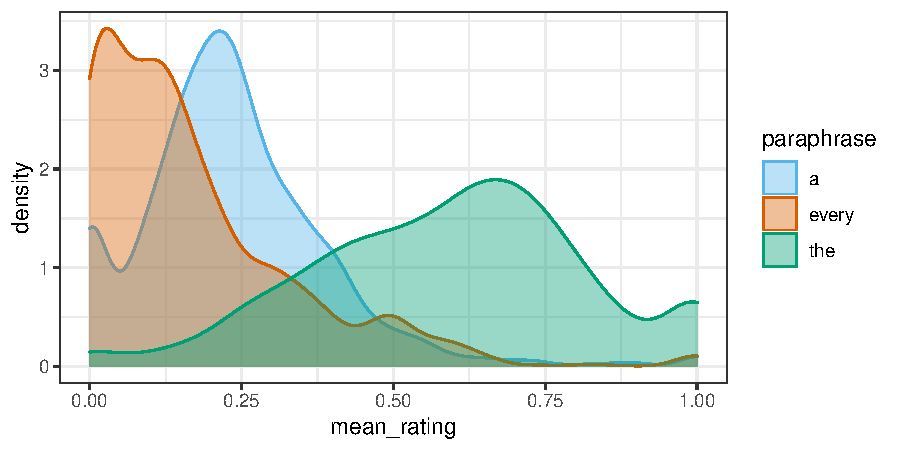
\includegraphics[scale=1]{figures/ex2b_denisty_mean_ratings.pdf}
\caption{Mean ratings by item for \emph{a}- and \emph{every}-paraphrases in Experiment 2b.}
\label{ex2b_density_mr}
\end{figure}

% \begin{figure}[h!]
% \centering
% 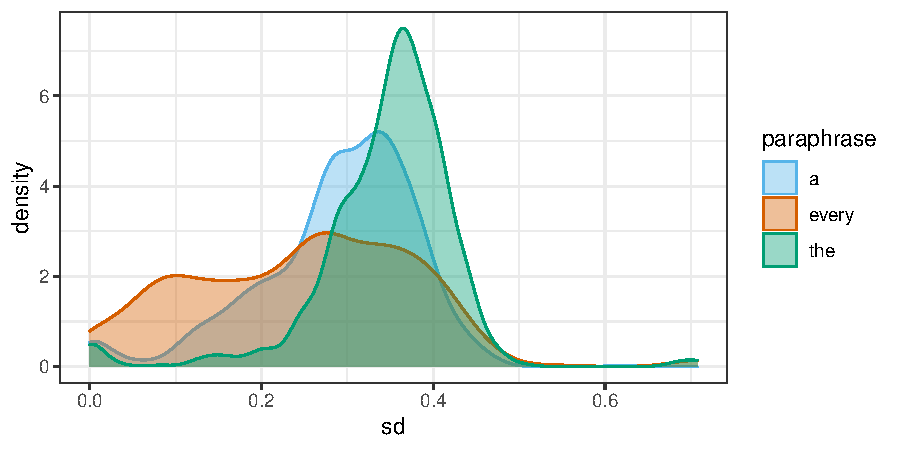
\includegraphics[scale=1]{figures/ex2b_denisty_sd.pdf}
% \caption{Standard deviations by item for \emph{a}- and \emph{every}-paraphrase in Experiment 2b.}
% \label{ex2b_density_sd}
% \end{figure}


\paragraph{Prediction 1: Is there an overall MA bias?}
\figref{ex2b_overall} plots mean rating as a function of paraphrase. No \whq revealed a significant initial bias for MA. In contrast, all \whqs except \emph{what}-questions revealed significant initial biases for MS paraphrases. 

\begin{figure}[h!]
\centering
\centering
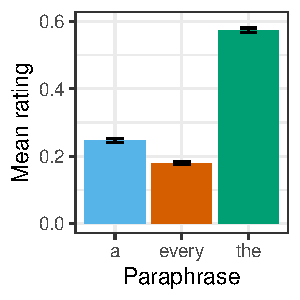
\includegraphics[scale=1]{figures/overall_nocontext_embedded.pdf}
\caption{Mean ratings by paraphrase in Experiment 2b. Here and below, error bars indicate 95\% bootstrapped confidence intervals.}
\label{ex2b_overall}
\end{figure}


\paragraph{Predictions 2, 3, and 5: Is MS modulated by the presence of modality, matrix verb, and \whw?}
\figref{ex2b_modXwh} plots mean rating as a function of ModalPresent, Wh-Word and Paraphrase. Unlike the previous three experiments, most questions patterned together in showing an MS bias, except \emph{what}-questions which were consistently MA skewed (although not to the point of significance). For all \whqs except \emph{when} and \emph{who}, the presence of a modal gave rise to a significant MS bias. 

\begin{figure}[h!]
\centering
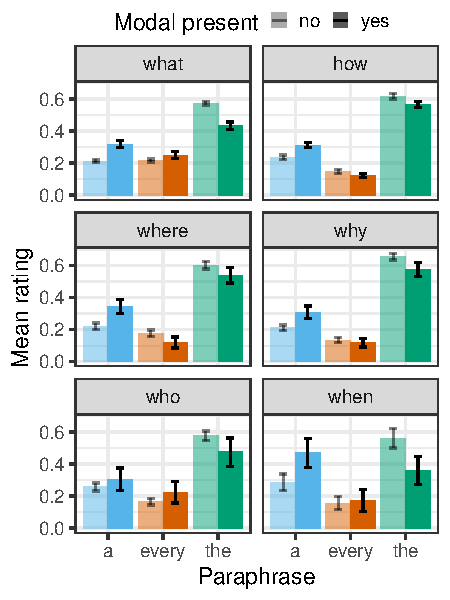
\includegraphics[scale=1]{figures/modxwh_nocontext_embedded.pdf}
\caption{Mean ratings by paraphrase, \whw and modality in Experiment 2b. Error bars indicate 95\% bootstrapped confidence intervals.} 
\label{ex2b_modXwh}
\end{figure}


\figref{ex2b_matrix_verbs} presents several matrix verbs that are of theoretical interest. As in Experiment 1b, we encounter sparse data problems and so focus on \emph{know-wh}. Before turning to those, we observe that with \emph{remember-wh}, 

\figref{ex2b_know_modXwh} presents meaning ratings for \emph{know-wh} questions as a function of paraphrase, Wh-Word and Modality. No \whq showed a bias for MA. Rather we found significant MS bias for \emph{know-how}: $\beta$=.16, $SE$=.02, $t$=8.97, $p<$0.0001 and \emph{know-where}: $\beta$=.12, $SE$=.03, $t$=3.65, $p<$0.0005; and an MS preference for \emph{know-what}, \emph{know-why}, \emph{know-who}, \emph{know-when}. The MS bias significantly increase with modality for \emph{know-what}: $\beta$=.01, $SE$=.04, $t$=3.19, $p<$0.002; \emph{know-how} $\beta$=.1, $SE$=.03, $t$=3.07, $p<$0.003, and \emph{know-where} $\beta$=.14, $SE$=.06, $t$=2.18, $p<$0.04, but not \emph{know-why}, \emph{know-who}, \emph{know-when}.

\begin{figure}[h!]
\centering
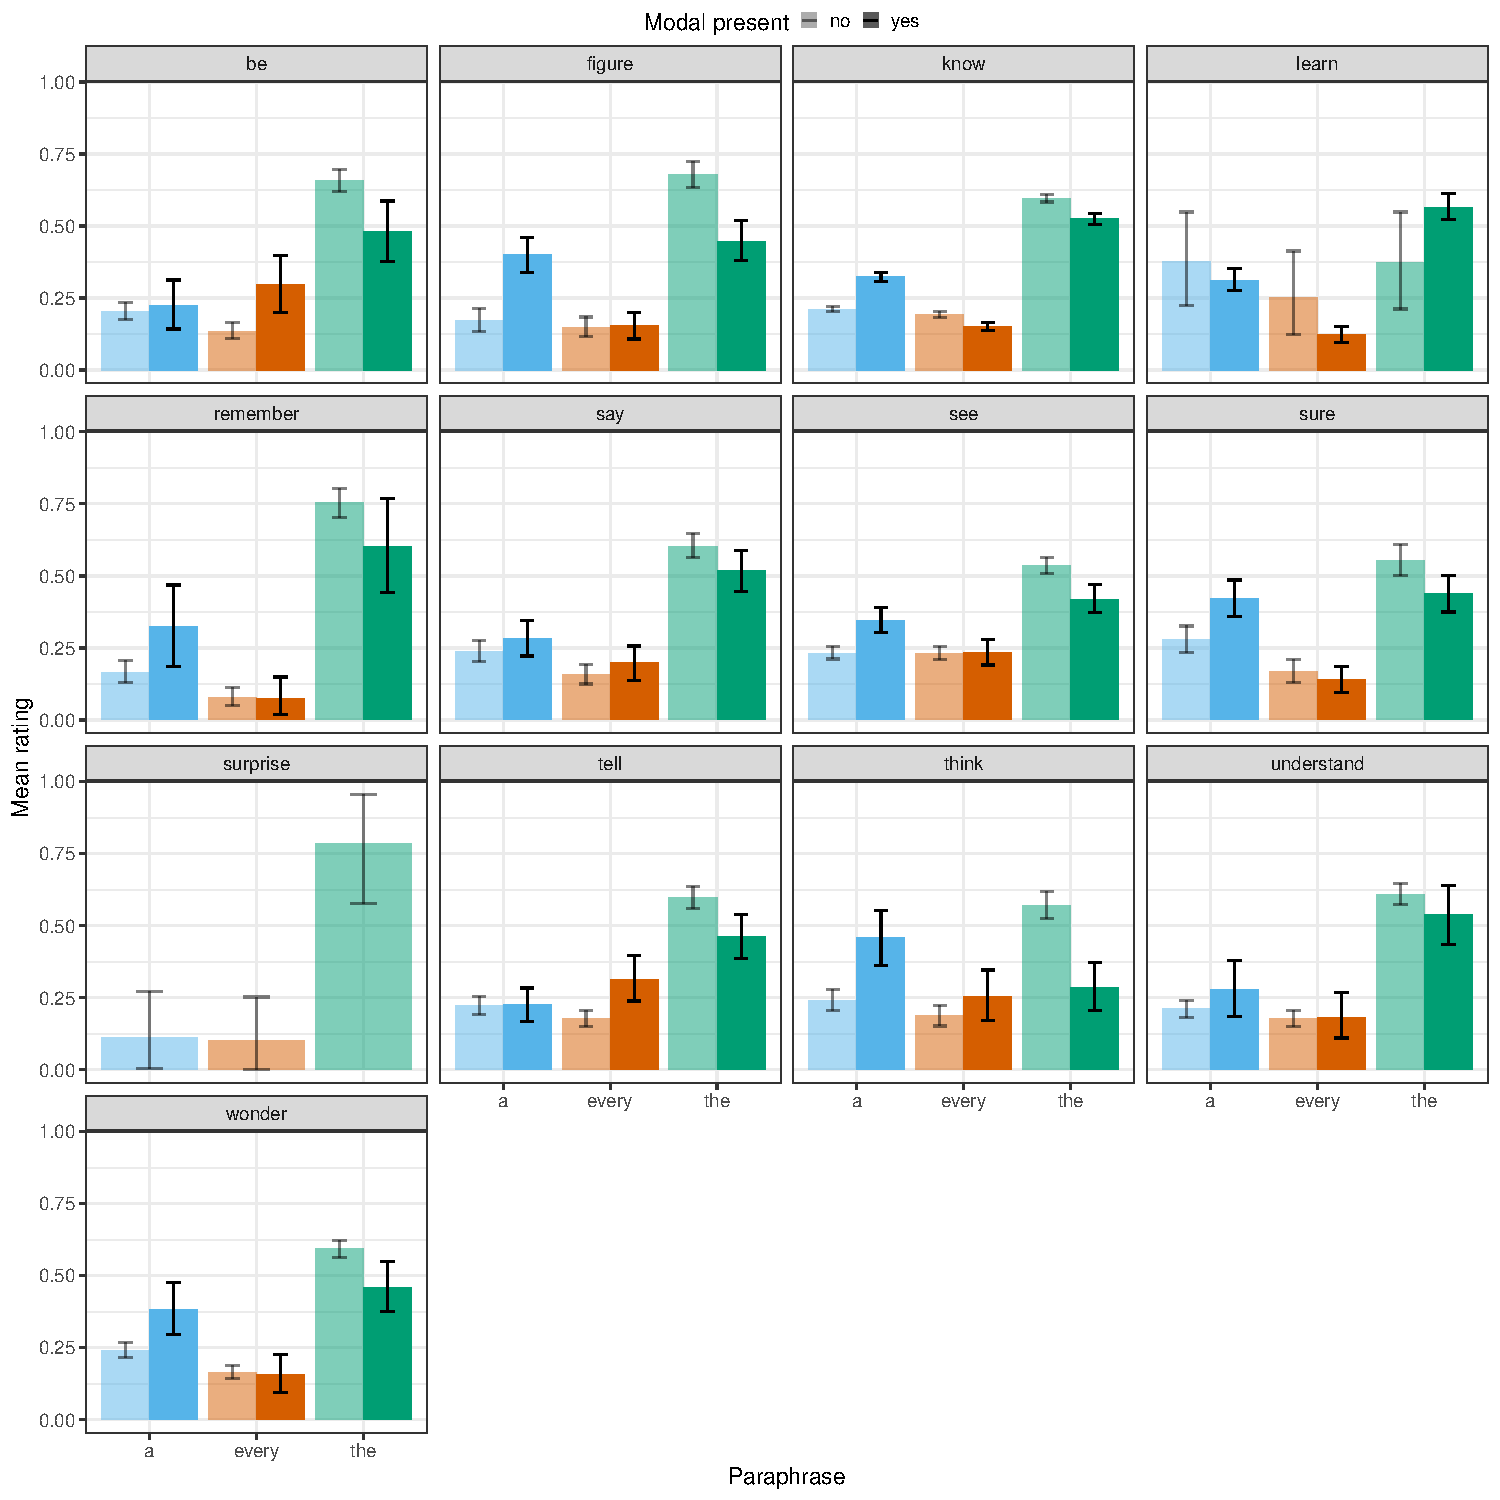
\includegraphics[scale=.6]{figures/matrixverbs_threotical_nocontext.pdf}
\caption{Mean ratings by paraphrase, \whw and modality in Experiment 2b. Error bars indicate 95\% bootstrapped confidence intervals.} 
\label{ex2b_matrix_verbs}
\end{figure}


\begin{figure}[h!]
\centering
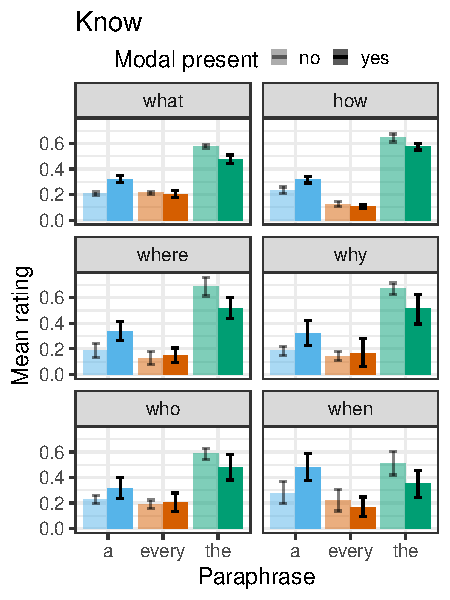
\includegraphics[scale=1]{figures/modwh_know_nocontext.pdf}
\caption{Mean ratings of questions embedded under \emph{know} as a function of paraphrase, \whw and modality in Experiment 2b. Error bars indicate 95\% bootstrapped confidence intervals.} 
\label{ex2b_know_modXwh}
\end{figure}


\subsection{Discussion}
We found that with the preceeding context removed, both root and embedded \whqs actually showed more bias for MS paraphrases than we expected. Theories which argue that only MS is context dependent would predict that MS readings should decrease without the proper contextual support. 

We still found interactions due to the lingusitic form of the question, although there were less robust effects of Modal present, as well as differences due to whether it was the root or the embedded task. For embedded \emph{what}-questions alone the presence of a modal reversed a non-significant MA bias, but there were no higher effects with root questions. For \emph{how}-questions, both root and embedded questions pattern together by exhibiting an MS bias that is strengthened by a modal. \emph{Where} and \emph{why}-questions patterned together: for root questions, there was significant MS bias but no influence of modality; for embedded questions the modal did signfifcantly increase the already significant MS bias. For root \emph{who}-questions there was only a significant interaction which raised MS ratings in the presence of modality; for embedded questions, there was significant bias for MS ratings but no effect of or interaction with modality. Finally, \emph{when}-questions showed no interactions between Paraphrase and ModalPresent, but significant positive biases for \emph{a}-paraphrases. Only with Root questions did modality boost MS.



\section{Prediction 4: Exploratory meta analysis assessing the effect of context}
How crucial is the role of context? In what ways does the presence/absence of explicit linguistic context change the distribution of paraphrases? 

If the discourse context provides information about the contextual speaker goals which are crucial to resolving question interpretation, then we should find that interpretation will be harder to resolve in the NoContext condition, where that crucial information is missing. This could manifest in different ways. In the face of this uncertainty about interpretation, participants might rely more on the linguistic form of the question which provides a cue to the speaker's goal. Thus we might expect to see stronger effects of linguistic factors in the NoContext task than in the Context task. To test this, we introduce Task as a predictor in a regression model over the entire data set, allowing us to quantify the effect of Task and interaction with Wh and ModalPresent. We specifically predict that the effects of Wh and Modality should be stronger in the NoContext Task than the Context Task.

It is also possible participants will be overall more uncertaint about the intended meaning exactly because information about the speaker goal is lacking. This would be reflected in the distributions of paraphrase ratings, where in the NoContext Task the  by-item distributions would be more uniform (reflecting that uncertainty) than in Context Task. To test this hypothesis, we compared the by-item distributions for each task to the uniform distribution using the Kullback-Leibler Divergence.


% On the one hand, we might expect that without contextual information, hearers would default to the minimal model of meaning that is provided by the semantics. On the other hand, we might expect that hearers would default to their expectation about what the likely goal that the speaker who utters the sentence would have had. 

\subsection{Qualitative discussion of examples}

We subtracted, for each item and paraphrase, the rating in the Context Task from the rating in the NoContext Task. In this section, we discuss some specific examples to help us understand what the effect of context is. 

\subsubsection{Cases with a big difference between the two studies}


\paragraph{For A-paraphrases} Let us first discuss examples where mean rating for \emph{a}-paraphrase was higher in the Context Task than in the NoContext Task. In some cases, ratings shifted clearly from \emph{a} in the context experiment to \emph{the} in the NoContext experiment.
\begin{exe}
\ex {}
\begin{xlist}
    \ex {}
    Speaker A: That's awful.\\
    Speaker B: And he goes out and commits it again. Fact, he's back in jail now. So, what, what, uh,\\
    Speaker A: Gives you sympathy for the vigilantes.\\
    Speaker B: \emph{What deterrent does he really have?}
    
    \ex \textbf{Rating distributions}:\\
    Context Task [a: .63, every: .16, the: .21]\\
    NoContext Task [a: .18, every: .17, the: .64]
    \end{xlist}
\end{exe}
What about the context makes a MS paraphrase better here? For avoiding jail, a single deterrent suffices, but it's not clear from the context that there exists one. Indeed, since the discussion is about recitivism in the relevant person, perphans the speaker is indicating that there exists no deterrent for this person. In contrast, without that information, we don't know what needs to be deterred, nor whether there is a salient deterrent that the speaker has in mind.

In other cases, probability mass shifted from \emph{a} to more evenly between both \emph{every} and \emph{the}:
\begin{exe}
    \ex {}
    \begin{xlist}
    \ex {}
    Speaker A: I mean, I'm just thinking of my circle of people that I know, I know quite a few people who have decided to not have both, both, both, uh, couples, you know, both, uh, of the parents work.\\
    Speaker B: yeah.\\
    Speaker A: and yet, uh, I, I we-, I hope to see employer based, you know, helping out. you know, child, uh, care centers at the place of employment and, and things like that, that will help out.\\
    Spealer B: uh-huh.\\
    Speaker A: \textbf{What do you think?}
    
    \ex \textbf{Rating distributions}:\\
    Rating Context Task [a: .43, every: .29, the: .27]\\
    Rating NoContext Task [a: .09, every: .4, the: .5]
    \end{xlist}
\end{exe}
The question \emph{What do you think?} is vague. The dialogue in which this question is occurring 






In yet other cases, there was a more even spread over the three paraphrases without context. Note that we predicted that removing context would introduce more uncertainty about the intended meanings, refelected in a flatter probability distribution in the NoContext Study. 
\begin{exe}
    \ex {}
    \begin{xlist}
    \ex {}
    Speaker A: Yeah what did you think about \emph{Dances with Wolves} when you saw it?\\
    Speaker B: Well, okay, see, we're getting back to last year. That's probably the last movie I saw. Um, \emph{Dances with Wolves}, I just adored it.\\
    Speaker A: Really?\\
    Speaker B: \textbf{How can I tell you?}
    
    \ex \textbf{Rating distribution}:\\
    Rating Context [a: .68, every: .03, the: .29]\\
    Rating Nocontext [a: .33, every: .23, the: .45] 
    \end{xlist}
\end{exe}
Here, context is providing information about what is being told, namely the extent to which Speaker B adored \emph{Dances with Wolves}. Without this information, the question is incredibly vague and it's not clear what the speaker is asking.



\paragraph{Examples where mean rating for \emph{a}-paraphrase was higher without Context} In other words, examples where other paraphrases received higher ratings in Contex than out.

Some theories argue that MS requires special contextual licensing. As minimal models of interpretation \emph{all else equal}, these theories predict that MS ratings should be reduced when that special contextual licensing is removed. The items in this section exemplify our finding that in fact, MS ratings increased in the NoContext Task contra theories mentioned above.ß

\begin{exe}
    \ex {}
    \begin{xlist}
    \ex {}
    Speaker A: We didn't, we didn't even think about it, you know.\\
    Speaker B: No. And now, you know, what do we have now. You know, got kids that, mumblex either got a, you know, a magnum gun school, like good grief.\\
    Speaker A: R-, right.\\
    Speaker B: I mean, I'd, I'd be afraid to be in school, I mean b-, teaching, or even being a student. \textbf{and think what, what's it going to be like for my, my youngest, and my oldest son, when he goes to school?}
    
    \ex \textbf{Rating Distribution}:\\
    Context Task [a: .14, every: .59, the: .27]\\
    NoContext Task [a: .77, every: .23, the: 0]
    \end{xlist}
\end{exe}
This context is about school shootings, a high-stakes context following the criterion of \citeA{moyersyrett2019}. Presumably, in these kinds of situations, a school will prioritize mapping out as many scenarios as possible so they can be prepared for any school shooter situation. Having exhaustive knowledge is the goal. 


\begin{exe}
    \ex {}
    \begin{xlist}
        \ex {}
        
        \ex \textbf{Rating Distribution}:\\
        Context Task [a: ., every: ., the: .]\\
        NoContext Task [a: ., every: ., the: .]
    \end{xlist}
\end{exe}


\begin{exe}
    \ex {}
    \begin{xlist}
        \ex {}
        
        \ex \textbf{Rating Distribution}:\\
        Context Task [a: ., every: ., the: .]\\
        NoContext Task [a: ., every: ., the: .]
    \end{xlist}
\end{exe}


\paragraph{For Every-paraphrases}

In some cases the probability mass shifted between \emph{every} and \emph{the}, and it was the Context task where \emph{every} was rated higher.
\begin{exe}
\ex {}
    \begin{xlist}
    \ex {}
    Speaker A: huh?\\
    Speaker B: \\
    Speaker A: uh-huh.\\
    Speaker B: \\
    Speaker A: I'm sure.\\
    Speaker B: Um, you look at your paycheck \textbf{and you go, oh, my gosh where did it all go?}
    \ex \textbf{Rating Distribution}:\\
    Rating Context [a: .07, every: .75, the: .19]\\
    Rating Nocontext [a: .21, every: .21, the: .59]
    \end{xlist}
\end{exe}

In this example, the context introduces \emph{paycheck} as the reference for \emph{it}. It is plausible that world knowledge about paychecks is to blame for the raise in the \emph{every} rating here. One doesn't spend one's paycheck (typically) at one single place, i.e., it typicallly is distributed over several places. In this sense, \emph{paycheck} isn't referring to a physical thing, but a collection of money. Note that, without the context, it makes sense that \emph{where did it all go?} would have a high \emph{the} rating, because the speaker appears to be referring to one thing going to one place. \mm{perphase, in part due to definiteness on the pronoun? find some citations like B\'uring?} The context introduces a more complex antecedent for the pronoun. \mm{It's also interesting to think about the function of \emph{all} in this example.}


\begin{exe}
\ex {}
    \begin{xlist}
    \ex {}
    Speaker A: Well, I, I, I think we did, I think we did learn some lessons that we weren't, uh, we weren't prepared for. I guess the best word would be the atrocities of war.\\
    Speaker B: Yeah.\\
    Speaker A: Uh, I mean the other wars seemed like a valiant war. I mean they seemed like a valiant thing.\\
    Speaker B: Yeah.\\
    Speaker A: \textbf{You know, you knew who was good}.
    
    \ex \textbf{Rating distribution}:\\
    Rating Context [a: .19, every: .6, the: .22]\\
    Rating Nocontext [a: .27, every: .1, the: .63]
    \end{xlist}
\end{exe}



There actually weren't many cases where \emph{every} was higher without context. The following is an example of one, but note that the in neither task is \emph{every} rated highest. Rather, \emph{a} is rated highest in the Context Task, and \emph{the} in the No-Context task.
\begin{exe}
\ex {}
    \begin{xlist}
    \ex {}
    Speaker A: and so there's only certain times you can talk to him. and\\
    Speaker B: and you could get there and his office hours could, i mean he could have like a nine to eleven in the morning office hours and have fourty-two people waiting to talk to him, and you still didn't get to talk to him anyway.\\
    Speaker A: right, yeah.\\
    Speaker B: \textbf{well, what would be your advice to a parent of a child thinking of attening college?}
    
    \ex \textbf{Rating distribution}:\\
    Rating Context [a: .44, every: .23, the: .33]\\
    Rating Nocontext [a: .28, every: .48, the: .24]
    \end{xlist}
\end{exe}




\paragraph{For The-paraphrases}

Cases where rating was higher in the Context task:

In most of these cases, participants were highly certain that the \emph{the} paraphrase was the one intended by the speaker in the Context experiment. In the NoContext experiment, they were less certain and we saw probability mass more evenly distributed between the three (although, often \emph{the} was still rated highest).

\begin{exe}
\ex {}
    \begin{xlist}
    \ex {}
    Speaker A: of course I would want one if somebody was given to me.\\
    Speaker B: yeah.\\
    Speaker A: but I maybe would buy a BMW. uh, or, even a Volvo.\\
    Speaker B: uh-huh.\\
    Speaker A: \\
    Speaker B: \textbf{What do you have now?}
    
    \ex \textbf{Rating distribution}:\\
    Rating Context [a: .02, every: .01, the: .96]\\
    Rating Nocontext [a: .25, every: .26, the: .49]
    \end{xlist}
\end{exe}

In this example, Context supplies the relevant domain of cars, in which typically people only have a single one. Even though \emph{the} is still highly rated in the NoContext task, note that probability is distributed almost evenly between \emph{a} and \emph{every}. 


\begin{exe}
\ex {}
    \begin{xlist}
    \ex {}
    Speaker A: and I did not like giving it out. I mumblex gave out my work number.\\
    Speaker B: Right.\\
    Speaker A: But I think I'm not sure if it's by law just, otherwise I think the practice has basically been eliminated asking for a phone number.\\
    Speaker B: Well, that's the thing I hate too about, uh, radio shack. \\
    Speaker A: \textbf{How did radio shack work?}
    
    \ex \textbf{Rating distribution}:\\
    Rating Context [a: .03, every: .08, the: .89]\\
    Rating Nocontext [a: .33, every: .21, the: .47]
    \end{xlist}
\end{exe}


In context, the question is clearly about policies on asking for phone numbers. Furthermore, the existential presupposition that Radio Shack has a policy on the topic is satisfied by Speaker B who explicitly has a (negatively valanced) attitude towards it. Without context, it's less clear which policy is the relevant one (i.e., \emph{work} in what respect?). It's less clear that the presuppositions of \emph{the} are satisfied, reflected in the fact that ratings for \emph{a} and \emph{every} are both higher than in the Context Task (although \emph{the} is still the highest). Participants are less confident that the \emph{the} paraphrase was the intended one. 

Cases where rating for \emph{the} was highest in the NoContext task often involved some variation on the question \emph{What do you think?}, which was often rated with an expremely high probability for \emph{the} in the NoContext task (at 1). In the Context task, probability mass was often evenly distributed between all three paraphrases.

\begin{exe}
\ex {}
    \begin{xlist}
    \ex {}
    Speaker A: yeah, that's okay.\\
    Speaker B: Well, that's what I mean like I didn't know what the diffference between Dukakis and Bush was.\\
    Speaker A: Uh-huh.\\
    Speaker B: you know, I didn't know anything about Bush or Dukakis.\\
    Speaker A: \textbf{so what do you think about, uh, what do you think about what you see on tv about them, like in the news or on the ads?}
    
    \ex \textbf{Rating distribution}:\\
    Rating Context [a: .32, every: .36, the: .32]\\
    Rating Nocontext [a: 0, every: 0, the: 1]
    \end{xlist}
\end{exe}


\begin{exe}
\ex {}
    \begin{xlist}
    \ex {}
    Speaker A: So long.\\
    Speaker B: Thanks a lot. \\
    Speaker A: Well, uh, ho-, how do you view this whole subject?\\
    Speaker B: \\
    Speaker A: are you, uh, one who feels like you have, have benefited from the change in, in roles in women? \textbf{or, or what do you think?}
    
    \ex \textbf{Rating distribution}:\\
    Rating Context [a: .26, every: .49, the: .24]\\
    Rating Nocontext [a: 0, every: 0, the: 1]
    \end{xlist}
\end{exe}

Here's a case where it seems the 10 preceeding lines included the end of one discussion as well as the actual discourse preceeding the target question.



\subsubsection{Cases where there was minimal change in rating between the two Tasks}

% \paragraph{For A-paraphrases}

Some cases there was no uncertainty, and no effect of context.
\begin{exe}
\ex {}
    \begin{xlist}
    \ex {}
    Speaker A: I need to make myself do that.\\
    Speaker B: Yeah. I slacked off a little because of, um, I'm about to graduate from college and so this past couple months have been really hectic so I haven't really gone and I've really been faithful these past two months of going to the health club and working out but...\\
    Speaker A: \textbf{What school you going to?}\\
    
    \ex \textbf{Rating distribution}:\\
    Rating Context [a: 0, every: 0, the: 1]\\
    Rating Nocontext [a: 0, every: 0, the: 1]
    \end{xlist}
\end{exe}


% \paragraph{For Every-paraphrases}

\begin{exe}
\ex {}
    \begin{xlist}
    \ex {}
    Speaker A: Generally cheap things.\\
    Speaker B: uh-huh.\\
    Speaker A: \\
    Speaker B: uh-huh\\
    Speaker A: \\
    Speaker B: uh-huh. yeah \textbf{we know how that goes}.
    
    \ex \textbf{Rating distribution}:\\
    Rating Context [a: .18, every: .1, the: .71]\\
    Rating Nocontext [a: .18, every: .11, the: .7]
    \end{xlist}
\end{exe}


% \paragraph{For The-paraphrases}

\begin{exe}
\ex {}
    \begin{xlist}
    \ex {}
    Speaker A: oh, yeah.\\
    Speaker B: and here's tis bum that didn't have a job.\\
    Speaker A: yeah.\\
    Speaker B: and he's got a attorney that you and i could never afford.\\
    Speaker A: that's true.\\
    Speaker B: \textbf{Who's paying for that?}
    
    \ex \textbf{Rating distribution}:\\
    Rating Context [a: .09, every: .07, the: .84]\\
    Rating Nocontext [a: .09, every: .07, the: .84]
    \end{xlist}
\end{exe}





\subsection{Results}

\figref{Task_overall} presents a comparison of the overal results from the Context task compared with the NoContext task. Overall, it seems that the distribution of ratings are largely similar between the two tasks; however, means are numerically higher in the NoContext Task for both \emph{a} (NoContext: mean=0.239, sd=.309, vs. Context: 0.216, 0.331) and \emph{the}-paraphrases (NoContext: mean=0.576, sd=.387, vs. Context: 0.547, 0.432) but the opposite for \emph{every}-paraphrases (Context: 0.237, 0.366, vs. NoContext: mean=0.185, sd=.303). 



\begin{figure}[h!]
\centering
\centering
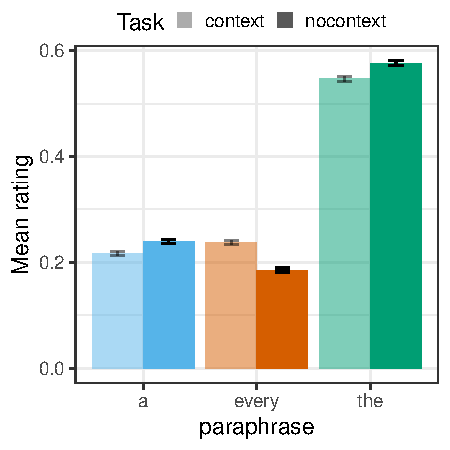
\includegraphics[scale=1]{figures/overall_Task.pdf}
\caption{Mean ratings by paraphrase comparing Context and NoContext Experiments.}
\label{Task_overall}
\end{figure}

We can see these differences from a slightly different angle in \figref{density_Task_overall}, which presents the mean by-item ratings for each paraphrase plotted as a function of Task. 
\begin{figure}[h!]
\centering
\centering
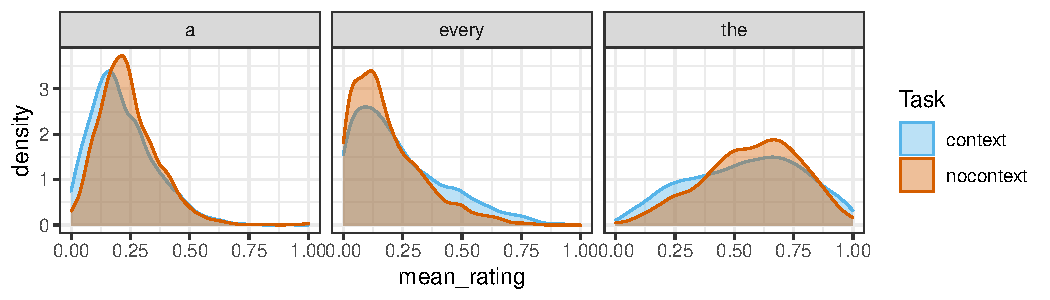
\includegraphics[scale=1]{figures/denisty_context_ratings.pdf}
\caption{Mean ratings by paraphrase comparing Context and NoContext Experiments.}
\label{density_Task_overall}
\end{figure}


\subsubsection{Regression analysis}
Some semantic theories predict that MS only requries special licensing by the context. Thus, if information that plays a licensing role is removed, it is plausible that those theories would predict that MS readings would decrease in the second set of experiments. We already saw that this prediction was not borne out. 

Analysis were conducted to assess the effect of Task (Context, NoContext) in addition to modality and \whw on question interpretation. Given the potential 4-way interaction by including Task as a predictor, we broke the data set up by Paraphrase and conducted three sub-model analysis.


\paragraph{The overall effect of Task on Paraphrase}

Table \ref{sub-model_Task} presents regression results assessing the effect of Context (Task) on \emph{a}- and \emph{every}- paraphrase ratings.
{}
% TASK COEFFICIENT TABLE
\begin{table}
\begin{center} 
\caption{Coefficient table (predicted $\beta$ coefficient, standard error $SE$, $t$ value, and $p$ value) for overall Task x Paraphrase model in metanalaysis comparing Context and NoContext tasks. Both predictors are dummy-coded and centered (0 is no Context and \emph{every}-paraphrase, 1 for Modal is present and \emph{a}-paraphrase.} 
\label{sub-model_Task} 
% \vskip .12in
\begin{tabular}{lllll} 
\toprule
{} & $\beta$ & $SE$ & $t$ & $p$\\
\midrule
Intercept & .22 & .003 & 80.66 & $<$.0001\\
Paraphrase & .01 & .006 & 2.26 & $<$.03\\
% \rowcolor{Gainsboro!100}
Task & -.01 & .003 & -4.75 & $<$.0001\\
% \rowcolor{Gainsboro!100}
Paraphrase:Task & .07 & .008 & 8.7 & $<$.0001\\
\bottomrule
\end{tabular} 
\end{center} 
\end{table}

\paragraph{\emph{A}-paraphrase Submodel}

\paragraph{\emph{Every}-paraphrase Submodel}


% TASK-A SUBMODEL COEFFICIENT TABLE
\begin{table}
\begin{center} 
\caption{Coefficient table (predicted $\beta$ coefficient, standard error $SE$, $t$ value, and $p$ value) for Task x ModalPresent \emph{wh}-word submodels for the data subsetted to \emph{a}-paraphrases. Both predictors are dummy-coded and centered (0 is no Context, 1 for Modal is present.} 
\label{sub-models_Task-a} 
% \vskip .12in
\begin{tabular}{l|lllll} 
\toprule
Wh-Word & {} & $\beta$ & $SE$ & $t$ & $p$\\
\midrule
WHAT & Intercept & .21 & .007 & 31.53 & $<$.0001\\
{} & ModalPresent & .1 & .01 & 11.15 & $<$.0001\\
% \rowcolor{Gainsboro!100}
{} & Task & .3 & .007 & 4.37 & $<$.0002\\
% \rowcolor{Gainsboro!100}
{} & ModalPresent:Task & -.03 & .01 & -2.86 & $<$.005\\
\bottomrule
\toprule
% HOW & $\beta$ & $SE$ & $t$ & $p$\\
% \midrule
HOW & Intercept & .25 & .006 & 42.91 & $<$.0001\\
{} & ModalPresent & .08 & .01 & 6.87 & $<$ .0001\\
% \rowcolor{Gainsboro!100}
{} & Task & .02 & .01 & 2.31 & $<$.05\\
% \rowcolor{Gainsboro!100}
{} & ModalPresent:Task & .001 & .01 & .07 & .94\\
% \bottomrule
\toprule
% WHERE & $\beta$ & $SE$ & $t$ & $p$\\
% \midrule
WHERE & Intercept & .22 & .02 & 14.7 & $<$.0001\\
{} & ModalPresent & .1 & .03 & 3.51 & $<$.0006\\
% \rowcolor{Gainsboro!100}
{} & Task & .01 & .02 & .8 & .44\\
% \rowcolor{Gainsboro!100}
{} & ModalPresent:Task & -.02 & .03 & -.75 & .46\\
\bottomrule
\toprule
% {} & WHY & $\beta$ & $SE$ & $t$ & $p$\\
% \midrule
WHY & Intercept & .22 & .007 & 32.84 & $<$.0001\\
{} & ModalPresent & .09 & .02 & 5.82 & $<$.0001\\
% \rowcolor{Gainsboro!100}
{} & Task & .02 & .01 & 1.27 & .24\\
% \rowcolor{Gainsboro!100}
{} & ModalPresent:Task & -.02 & .02 & -.67 & .5\\
\bottomrule
\toprule
% WHO & $\beta$ & $SE$ & $t$ & $p$\\
% \midrule
WHO & Intercept & .26 & .03 & 9.12 & $<$.0001\\
{} & ModalPresent & .12 & .04 & 2.92 & $<$.005\\
% \rowcolor{Gainsboro!100}
{} & Task & .04 & .01 & 2.87 & $<$.04\\
% \rowcolor{Gainsboro!100}
{} & ModalPresent:Task & -.03 & .04 & -.81 & .42\\
\bottomrule
\toprule
% WHEN & $\beta$ & $SE$ & $t$ & $p$\\
% \midrule
WHEN & Intercept & .27 & .03 & 9.25 & $<$.0001\\
{} & ModalPresent & .22 & .07 & 3.44 & $<$.002\\
% \rowcolor{Gainsboro!100}
{} & Paraphrase & -.01 & .03 & -.31 & .77\\
% \rowcolor{Gainsboro!100}
{} & ModalPresent:Paraphrase & -.01 & .06 & -.24 & .81\\
\bottomrule
\end{tabular} 
\end{center} 
\end{table}



% TASK-EVERY SUBMODEL COEFFICIENT TABLE
\begin{table}
\begin{center} 
\caption{Coefficient table (predicted $\beta$ coefficient, standard error $SE$, $t$ value, and $p$ value) for Task x ModalPresent \emph{wh}-word submodels for the data subsetted to \emph{every}-paraphrases. Both predictors are dummy-coded and centered (0 is no Context, 1 for Modal is present.} 
\label{sub-models_Task-every} 
% \vskip .12in
\begin{tabular}{l|lllll} 
\toprule
Wh-Word & {} & $\beta$ & $SE$ & $t$ & $p$\\
\midrule
WHAT & Intercept & .28 & .02 & 16.09 & $<$.0001\\
{} & ModalPresent & .05 & .02 & 3.05 & $<$.003\\
% \rowcolor{Gainsboro!100}
{} & Task & -.08 & .01 & -6.26 & $<$.0001\\
% \rowcolor{Gainsboro!100}
{} & ModalPresent:Task & .003 & .01 & .22 & .82\\
\bottomrule
\toprule
% HOW & $\beta$ & $SE$ & $t$ & $p$\\
% \midrule
HOW & Intercept & .17 & .01 & 14.83 & $<$.0001\\
{} & ModalPresent & -.01 & .01 & -.84 & .4\\
% \rowcolor{Gainsboro!100}
{} & Task & -.04 & .01 & -4.02 & $<$.0007\\
% \rowcolor{Gainsboro!100}
{} & ModalPresent:Task & -.002 & .01 & -.19 & .85\\
% \bottomrule
\toprule
% WHERE & $\beta$ & $SE$ & $t$ & $p$\\
% \midrule
WHERE & Intercept & .19 & .02 & 8.01 & $<$.0001\\
{} & ModalPresent & -.04 & .04 & -.97 & .34\\
% \rowcolor{Gainsboro!100}
{} & Task & -.04 & .01 & -.422 & $<$.0001\\
% \rowcolor{Gainsboro!100}
{} & ModalPresent:Task & .03 & .03 & 1.03 & .3\\
\bottomrule
\toprule
% {} & WHY & $\beta$ & $SE$ & $t$ & $p$\\
% \midrule
WHY & Intercept & .15 & .01 & 17.2 & $<$.0001\\
{} & ModalPresent & -.001 & .02 & -.06 & .95\\
% \rowcolor{Gainsboro!100}
{} & Task & -.03 & .01 & -2.95 & $<$.005\\
% \rowcolor{Gainsboro!100}
{} & ModalPresent:Task & -.01 & .02 & -.62 & .54\\
\bottomrule
\toprule
% WHO & $\beta$ & $SE$ & $t$ & $p$\\
% \midrule
WHO & Intercept & .23 & .02 & 10.35 & $<$.0001\\
{} & ModalPresent & .004 & .07 & .07 & .95\\
% \rowcolor{Gainsboro!100}
{} & Task & -.09 & .02 & -4.2 & $<$.002\\
% \rowcolor{Gainsboro!100}
{} & ModalPresent:Task & -.03 & .05 & -.49 & .62\\
\bottomrule
\toprule
% WHEN & $\beta$ & $SE$ & $t$ & $p$\\
% \midrule
WHEN & Intercept & .16 & .04 & 4.31 & $<$.004\\
{} & ModalPresent & .02 & .06 & .31 & .76\\
% \rowcolor{Gainsboro!100}
{} & Paraphrase & -.02 & .02 & -1.01 & .28\\
% \rowcolor{Gainsboro!100}
{} & ModalPresent:Paraphrase & .03 & .04 & .71 & .48\\
\bottomrule
\end{tabular} 
\end{center} 
\end{table}





% \mm{add in the model results from breaking it up by paraphrase}

\subsubsection{Quantifying information loss with KL divergence}


In addition to comparing 
We calculated the Kullback-Leibler Divergence from each Task and the uniform distribution over paraphrases to determine whether information about interpretation was lost in the NoContext Task, and conducted a regression analysis to determine whether Task predicted the KL divergence score.

We found that removing the context significantly decreased the KL-divergence score, meaning that ratings in the NoContext Task were closer to the uniform distribution, that information was lost when the context was removed.

% \mm{graph the KL divergence}

\begin{figure}[h!]
\centering
\centering
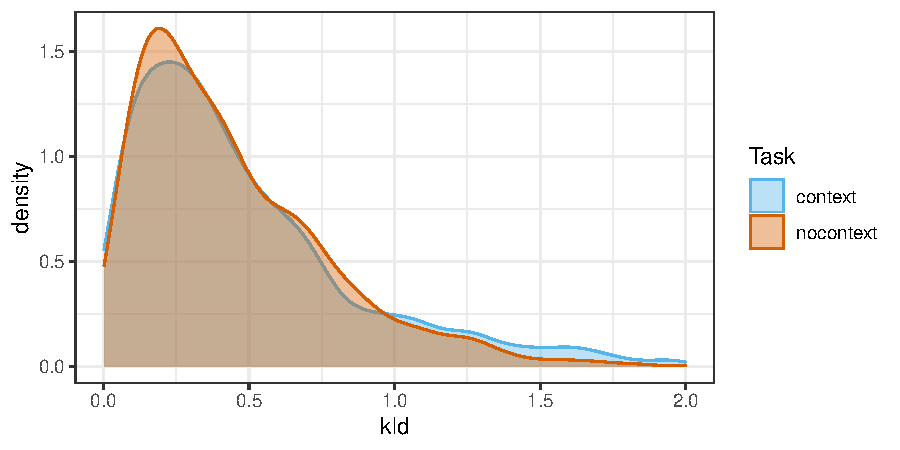
\includegraphics[scale=1]{figures/denisty_kld_context.pdf}
\caption{Mean ratings by paraphrase comparing Context and NoContext Experiments.}
\label{density_kld_overall}
\end{figure}


\subsection{Discussion}
We found that effects of Task were significant for Wh-Word, but not for Modality, suggesting that context is informative wrt the wh-domain which importantly helps determine the meaning that the speaker intended.  \jd{nice if true}


\subsection{Annotation of context for domain-relevant information}
We annotated a random sample of contexts of questions that rated high for MS for features that were relevant to determining the size and type of the \emph{wh}-domain. \jd{what is the point of this?}

\section{General Discussion}

We presented four experiments designed to test the distribution of (non-)exhaustivity in \whqs in naturally occurring speech. Experiments 1a and 2a investigated root questions, while Experiments 1b and 2b investigated questions embedded under propositional attitude verbs \jd{were they all propositional attitude verbs, not embedding predicates in general?}. To test the effect of contextual information on interpretation, Experiments 1a/1b presented targets with the immediately preceding dialogue, while Experiments 2a/2b presented targets without.


\jd{briefly summarize the results here in 3 sentences or so.}



\jd{this next paragraph deserves its own sub-section, should have a heading like "Implications for theories of \whqs", and contain explicit arguments. you can't just claim that the semantic rep is only existential -- you have to say why. you can't just claim that the interpretive process is bayesian -- you have to say why (and in fact, we don't have any evidence to that effect from the data presented here, so it's best to just leave this out, or instead frame as a promising direction for how to excplicitly model in-context reasoning about exhaustivity)}

\subsection{Implications for semantic theories of}
Givn our results, we argue that the semantic representation of a question is maximally underspecified or really weak, existential in meaning. The interpretive process of resolving that underspecification is Bayesian, and involves joint reasoning about the linguistic signal and its possible alternatives, in addition to the contextual speaker's goal.



\subsection{Limitations}

In our investigation of the linguistic surface features that predict question interpretation, we focused on three  that have been widely discussed in the literature: modality, \whw, and matrix verb. We saw that while these are predictive of exhaustivity in ways predicted by previous work \jd{cite cite}, in support of claims that variability in exhaustivity is at least to some extent semantically conditioned, we also observed both significant deviations from predictions as well as interactions between factors suggesting that at least some ``semantic'' effects are in fact defeasible pragmatic ones. \jd{my first stab at this, can be edited of course.} 

However, there are other linguistic factors which we did not include in our analyses, and which, if included, would have fully determined the results. \jd{rephrase, jd} 

\paragraph{Modality}
First, we used a coarse-grained measure of modality that included  modal auxiliaries and  non-finite clauses in embedded questions, but did not account for modal force and flavor (\cite{kratzer1981,kratzer1991,portner2009}). The semantics literature on the effect of modality on MS typically has focused on the existential priority modal \emph{can} as it has occured in the classic example, \emph{Where can I find an Italian newspaper?} On the one hand, we might predict that any modal with existential force would allow for MS because it's the existential bit that drives the MS meaning. This would put the modal observation squarely in line with the observation that existential items in the \whq generally lead to more MS readings than not. It is also concordant with theoretical accounts which argue, either that there is an implicit quantificational variation in the \whq \cite{hintikka1976,lahiri2002}, underlying existential quantification that can be strengthened with contextual information \cite{asherlascarides1998}.


There is a 

\jd{this was just getting interesting! :) would love to see where this is going}

\paragraph{In/definiteness}
Second, definite and indefinite noun phrases may reveal interesting differences with respect to MS and MA. On the one hand, \jd{what has been said about definiteness?}

\paragraph{Other \emph{Wh}-phrases}
Third, we chose to include only monomorphemic \emph{wh}-phrases, and not include questions with singular or plural marked \emph{wh}-phrases. \jd{remind us why} 

Similarly, we did not include clefts or relative clauses. There is a question in the literature on clefts about the extent to which they allow for non-exhaustive readings \mm{more citations?..check diss, devaug-geiss, zimmermann, destruel}. \jd{i don't think this needs to be listed as a limitation. instead, the connection to variability in cleft/relative clause interpretation can be mentioned in one sentence elsewhere}


Better that pragmatics is not sufficient: \jd{don't understand the point of these examples}
(discussion from George 205-206)
questions with ostensibly the same semantic representation 
\begin{exe}
\ex {}
    \begin{xlist}
        \ex Who has leprosy?
        \ex Who are some people with leprosy?
    \end{xlist}
\end{exe}
But we can question indeed whether these two questions would be asked by a speaker iwth the same goals in mind?


\paragraph{Question Type}

\jd{not sure i get what is being said in this section. here i would just focus on the fact that it's hard to actually assess the diffs between root and embedded questions because, with the exception of "know", we have huge data sparisity issues}

Fourth, we did find some differences between root and embedded questions. Embedded questions appeared to slightly prefer MA paraphrases over MS paraphrases, while root questions showed the opposite. This effect could be due to the additional effect of Matrix verb which was not present for Root Questions. Indeed, the majority of embedded questions occured with the verb \emph{know}, which is classically MA. Additionally, there were some cases of embedded questions in which the question contained subject-auxiliary inversion, a connonical root question syntax. Some have argued that MS, being pragmatic, should not be possible in embedded questions (\cite{karttunen1977}\mm{footnote 4}, \cite{groenstok1984}\mm{footnote 14}, \mm{xiang?})

Of course, this kind of ``pragmatics does not interfere in semantics'' view is less in vogue than it used to be, in part because of the growing understanding of pragmatic processing (\mm{reference list from kreiss \& degen cog sci paper}). We did an exploratory analysis on the effect of Question Type (true embedded, embedded with subject-aux inversion, true root) and the effects were not overwhelmingly different. \mm{Show graphs? do regression?} 


\paragraph{Corpus Genre}

\jd{why should corpus genre matter? be explicit}
The Switchboard corpus is comprised of conversational dyads between randomly assigned employees of Texas Instrunmnets. The conversants were strangers so they did't share a lot of common ground. There are at least two ways in which this affected the corpus. First, it affected the kind of questions asked, 

and second, it affected the 

Already, the fact that \whq interpretation could be sensitive to all these further factors suggests that 

\subsection{MISC discussion points}

Before continuing, let us pause for a terminological clarification. For root questions, we speak of MS/MA answers, while for embedded questions, we speak of MS/MA readings or interpretations. The distinction is often theoretically driven. `Answer' specifically means an element that fills in for the information missing from the \whq. For example, while \emph{I don't know} is a perfectly acceptable response to (\ref{coffee1}), it would not count as a answer; in contrast, coffee shop names do fill in the missing \emph{where} information in the right way. So `answer' is a technical notion.

In the embedded case, we use `reading' or `interpretation' because sentences with embedded \whqs do not have interrogative illocutionary force and thus no answers in the speech act sense. Although, semanticists do speak of `answers' to embedded question, using the technical notion described above. Yet here, `answers' aren't construed as assertions in the way they are with the root questions. Further, the difference between `reading' and `interpretation' is usually theoretically important. `Reading' implies an underlying semantic representation that determines the truth (answerhood) conditions, while `interpretation' applies more generally without commitment to an underlying representation. `Interpretation' often suggests that some other mechanism (usually pragmatic in nature) has intervened to cause the appearance of the data in question. Thus, some might reject the availability of MS \emph{readings} of some embedded questions, but acknowledge the possibility of MS \emph{interpretations} of them, given other (non-semantic) factors. Referring to an MS/MA \emph{reading} of a root question implies that an MS or MA answer suffices as a complete (and resolving) answer to the question. Referring to an MS/MA \emph{interpretation} of a root question implies that a language user has determined that an MS or MA answer is acceptable (though possibly incomplete or unresolving) for a root question, given the exigencies of context. Again, the distinction often boils down to the involvement of non-linguistic processes. 


\section{Conclusion}

\jd{i imagine all the stuff that follows is intended to be used in some form either in the intro or in the gd, but the conclusion should just be short and sweet}

Human communication proceeds remarkably fast and robustly despite the rampant underspecification of speakers' utterances with respect to the meaning they intend to convey. Resolving that underspecification requires that hearers integrate a wide range of possibly uncertain linguistic and extra-linguistic cues. 

This view of pragmatics, informed by psycholinguistic research on language processing that espouses a dynamic, nonmodular view of comprehension, has provided a useful novel perspective on many phenomena at the semantics/pragmatics interface. For instance, one of the most-studied cases of underspecification in experimental pragmatics is the scalar inference from \emph{some} to \emph{not all} (e.g., \emph{Scully ate some of the cookies} typically licenses the inference that she did not eat all of them). Recent research using a large dataset of naturally-occurring utterances has revealed a large amount of variability in whether hearers derive scalar inferences \cite{degen2015}. Rather than being random, the observed variability was dependent on multiple features of the linguistic and discourse context. Data from controlled experimental tasks with artificially generated stimuli confirm these results: scalar inferences are systematically dependent on (the hearer's estimate of) the speaker's discourse goal \cite{zondervan2010}\mm{kursatdegen2020}, the speaker's epistemic state \mm{goodmanstuhlmueller2013}\cite{brehenyetal2013}, and which alternatives are contextually available \cite{huangsnedeker2011,degentanenhaus2016}, among other cues. These results were unexpected in light of the theoretical literature, which had predicted a higher prevalence of the inference and no systematic context-dependence \cite{levinson2000}.

A good deal of experimental attention has been paid to pragmatic inferences, like scalar inferences, that are the result of reasoning about declarative utterances. In contrast, there is much less discussion about the cues guiding hearers' interpretation of non-declarative utterances like questions. Consider polar (\emph{yes}-\emph{no}) questions: these can be answered literally with a \emph{yes} or \emph{no}, but often the literal answer is neither the most appropriate, nor what the speaker intended. In \citeA{searle1975}'s classic example, a dinner guest who asks \emph{Can you reach the salt?}~likely intends you to pass the salt, not say \emph{yes}. Whether a hearer understands the speaker to want a literal or non-literal answer depends on what they infer about the speaker's goals. \citeA{clark1979} surveyed liquor merchants to determine how they answered a polar question like \emph{Does a fifth of Jim Beam cost more than \$5?} when it was introduced by a brief sentence that made the speaker's goal explicit. If the speaker first stated \emph{I want to buy some bourbon}, merchants were more likely to answer with the exact price of the whiskey. If the speaker instead stated \emph{I've got \$5 to spend}, merchants were more likely to provide the more literal \emph{yes}/\emph{no} answer. That is, merchants responded by addressing the inferred speaker goal. Research in computational cognitive science has followed suit by modeling question asking and answering as a species of rational, goal-directed behavior \cite{hawkinsetal2015,rotheetal2018}. \mm{hawkinsgoodman2019?}\emph{Wh}-questions are even more complex than polar questions in that even their literal interpretation is underspecified. 




\bibliographystyle{apacite}

\setlength{\bibleftmargin}{.125in}
\setlength{\bibindent}{-\bibleftmargin}

\bibliography{questions}

\end{document}